\documentclass[10pt,a4paper]{article}
\usepackage[utf8]{inputenc}
\usepackage[frenchb]{babel}
\usepackage[T1]{fontenc}
\usepackage{graphicx}
\usepackage{fancyhdr}
\usepackage{eurosym}

\lhead{Créer facilement son site Internet avec Wordpress}
\rhead {Rémy Mondi (iMaugis)}
\lfoot{
\includegraphics[scale=0.5]{img/cc-by-nc-sa.png}}
\cfoot{}
\rfoot{Page \thepage}

\pagestyle{fancy}

\title{Créer facilement son site Internet avec Wordpress}
\author{Rémy Mondi (iMaugis)}
\date{\today}

\begin{document}

\maketitle
\begin{figure}[!h]
\begin{center}

\includegraphics[scale=0.5]{img/logo-wordpress.png}
\end{center}
\end{figure}
\newpage

\tableofcontents
\newpage

\part{Qu'est-ce que Wordpress?}
\newpage
\paragraph{} \begin{center}\textit{La définition ci-dessous est extraite du cours "Propulsez votre site avec Wordpress" issu du site OpenClassrooms}\end{center}
\section{Introduction}
\paragraph{}Aujourd'hui, de nombreux acteurs du monde informatique se sont mis à la mode des blogs, ces petits sites de contenu gérés la plupart du temps par une personne et qui laissent transparaitre les réflexions de leur auteurs sur les sujets qui les passionnent. Pour faciliter la création de ces sites d'un genre particulier, il est préférable de partir d'un système solide et qui a fait ses preuves, tout en évitant aux auteurs les complications du développement d'un site Internet.
\paragraph{}WordPress est un est un logiciel libre qui a été créé dans cette optique, c'est donc probablement l'outil qu'il vous faut si vous désirez tenir un blog ou bien simplement un site de présentation personnel ou d'entreprise. Bien qu'il soit principalement spécialisé dans la création de blogs, c’est cependant loin d’être sa seule possibilité et rien ne vous empêchera de créer un site différent.
\paragraph{}Ainsi, il est bon à savoir que WordPress est un CMS (Content Management System ou Système de Gestion de Contenu en français), c’est-à-dire qu’il permet à l’utilisateur (c'est-à-dire l’administrateur du site) de créer facilement des pages de contenu, comme par exemple :
\begin{itemize}
\item la page de présentation d’une entreprise ;
\item des articles de blog ;
\item une page de contact ;
\item un portfolio pour un artiste ;
\item bien encore des fiches produits sur un site de vente en ligne ;
\item etc...
\end{itemize}
\paragraph{}L’idée d’un CMS est de donner la possibilité de facilement créer du contenu sur le site, sans avoir à mettre les mains dans le code ni même avoir de connaissances techniques particulières.
\section{Historique}
\paragraph{}WordPress est sorti pour la première fois en 2003 comme un projet dérivé de cafelog, lui-même étant un moteur de blog sorti en 2001. De nombreuses versions sont sorties depuis, chacune apportant son lot de nouveautés par rapports aux versions précédentes, comme les plugins, les widgets, les thèmes, une interface utilisateur améliorée… La version 3 est sortie en 2010 en apportant notamment la gestion des menus, de nouvelles fonctions pour gérer l’en-tête du site ainsi que le support du multisite (c’est ce qui permet d’avoir plusieurs sites sur une même instance de WordPress).
\section{Fonctionnalités}
\paragraph{}WordPress est écrit en PHP, un langage de programmation spécialisé dans la création de sites Internet. Ce langage permet donc aux développeurs de rajouter des fonctionnalités qui pourront être réutilisées par d’autres utilisateurs. Il est donc facile à modifier si vous avez de bonnes bases dans ce langage.
\paragraph{}L’une des grandes forces de WordPress est ainsi la multitude de plugins disponibles, développés par la communauté. Ce sont des modules permettant d'ajouter des fonctionnalités à WordPress, comme par exemple la création d'une galerie photo ou la gestion d'une newsletter. Il y en a aujourd’hui plus de 25 000 plugins sur le site officiel, wordpress.org. Il y a donc fort à parier que, si vous cherchez une fonctionnalité supplémentaire pour votre site, un plugin existe déjà pour cela ! Si cela n’était pas le cas, vous pouvez bien entendu développer le votre et éventuellement le publier.
\paragraph{}La renommée de WordPress dans le monde du blogging est telle qu’il existe même un site dédié, wordpress.com (à ne pas confondre avec le site officiel en .org), qui vous permet de créer votre blog WordPress sans vous occuper de son hébergement ou de son installation. Tout est géré automatiquement, vous n’avez qu’à créer votre contenu. Vous n’avez en revanche pas directement la main sur le code et il sera nécessaire de passer par l’installation de thèmes ou de plugins pour faire des modifications fonctionnelles.
\newpage

\part{Installer Wordpress}
\newpage

\section{Où trouver Wordpress?}
\subsection{Télécharger Wordpress}
\paragraph{}Démarrez votre navigateur et rendez-vous à l'adresse suivante :
\paragraph{}http://fr.wordpress.org/
\begin{center}
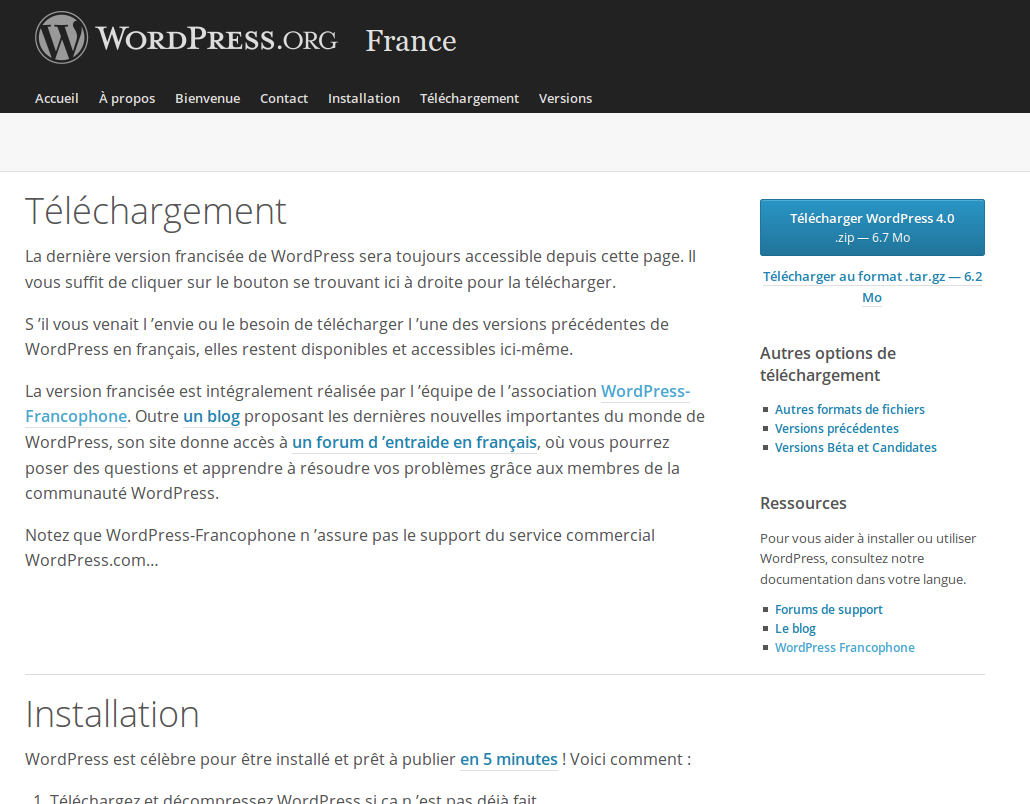
\includegraphics[scale=0.35]{img/0001.png}
\end{center}
\paragraph{}Cliquez sur le bouton « Téléchargez WordpressX.X ».
\begin{center}
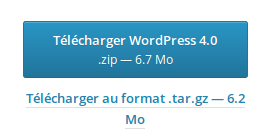
\includegraphics[scale=0.7]{img/0002.png}
\end{center}
\paragraph{}Dans la boîte de dialogue qui apparaît, sélectionnez « Enregistrer le fichier » (ou équivalent suivant votre navigateur) puis cliquez sur « Ok ».
\begin{center}
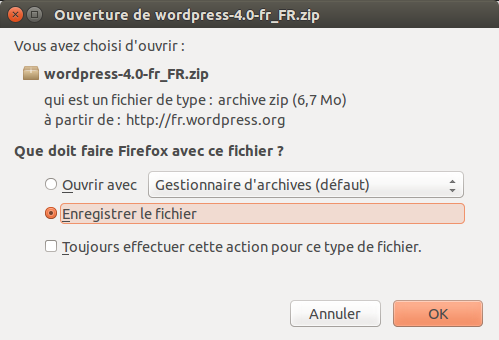
\includegraphics[scale=0.5]{img/0003.png}
\end{center}
\paragraph{}Le téléchargement se lance...
\paragraph{}Et voilà ! Vous avez téléchargé Wordpress qui doit désormais se situer dans le dossier « Téléchargements » de votre répertoire personnel sous la forme d'une archive compressée nommée wordpress-x.x-fr\_FR.zip.
\subsection{Décompresser l'archive téléchargée}
\paragraph{}Rendez-vous dans le dossier « Téléchargements » de votre répertoire personnel.
\paragraph{}Faites un clic-droit sur l'archive wordpress-x.x-fr\_FR.zip puis, dans le menu contextuel qui apparaît, cliquez sur « Extraire ici ».
\begin{center}
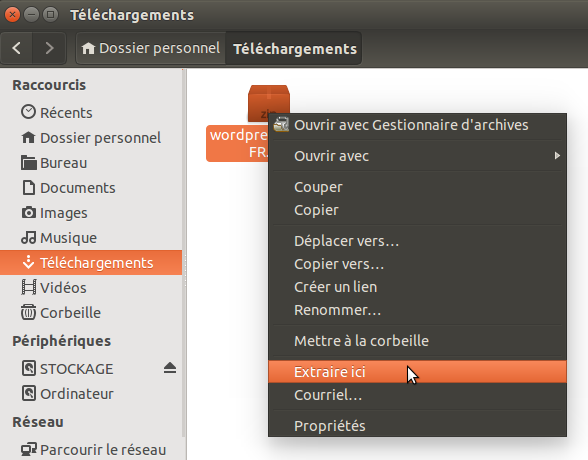
\includegraphics[scale=0.5]{img/0004.png}
\end{center}
\paragraph{}L'archive est désormais décompressée, vous pouvez observez tous les dossiers et fichiers composant Wordpress (comme ci-dessous) :
\begin{center}
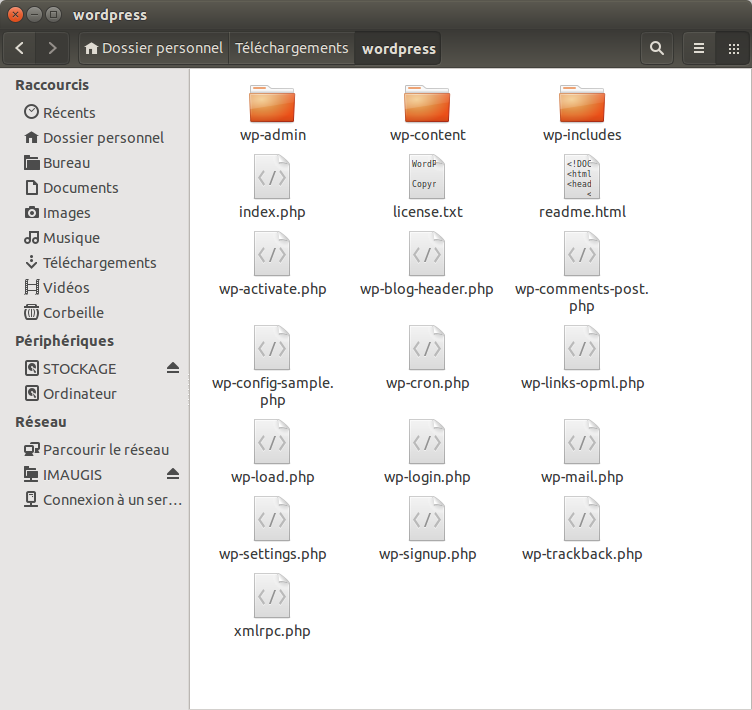
\includegraphics[scale=0.4]{img/0005.png}
\end{center}
\newpage

\section{Héberger son site Wordpress}
\subsection{Qu'est-ce qu'un hébergement?}
\paragraph{}Comme expliqué lors de la première session, tout bon site qui se respecte est « hébergé » sur un serveur. Les serveurs ne sont ni plus ni moins que des ordinateurs améliorés (matériel plus performant et plus solide) qui sont allumé 24h/24 et 7 jours / 7. Ils sont en général regroupés dans des lieux qu'on appelle des Data Center. Le rôle des serveurs est... de servir ! En l'occurrence dans notre cas de permettre à notre site Wordpress d'être accessible à tous moments par vos futurs visiteurs en entrant simplement l'adresse web du site (appelé aussi nom de domaine) ou en effectuant une recherche via un moteur de recherche (Google, Yahoo, etc...).
\begin{center}
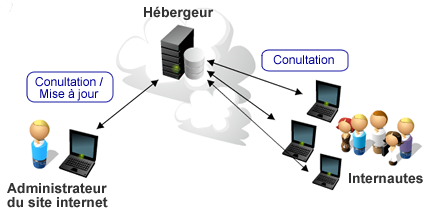
\includegraphics[scale=0.5]{img/0006.png}
\end{center}
\paragraph{}Mais louer ou mettre en place un serveur web n'est pas chose aisée et il faut des compétences spécifiques afin d'accomplir cette tâche.
\paragraph{}Heureusement pour nous, il existe une autre solution qui ne nécessite que peu de compétences : l'hébergement dit « mutualisé ».
\paragraph{}En effet un hébergement mutualisé est une parcelle allouée sur un serveur. Plusieurs sites Internet peuvent donc se partager le même serveur web (d'où le terme mutualisé).
\begin{center}
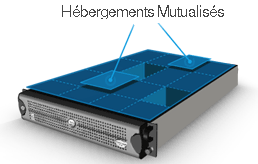
\includegraphics[scale=0.5]{img/0007.png}
\end{center}
\paragraph{}Les avantages de cette solution sont nombreux :
\begin{itemize}
\item Coûts faibles
\item Toutes les interventions techniques sont à la charge de l'hébergeur
\item Aucune connaissance d'administration requise
\item Nombreux services annexes inclus (nom de domaine, comptes email, etc...)
\end{itemize}
\paragraph{}C'est pourquoi nous vous conseillons cette solution pour héberger votre site Wordpress !
\paragraph{}Voir les offres : https://www.ovh.com/fr/hebergement-web/
\subsection{Un Hébergement mutualisé abordable : OVH}
\paragraph{}Vous trouverez chez OVH des offres d'hébergement mutualisé très fiables et tout à fait abordables pour le budget d'une association.
\begin{center}
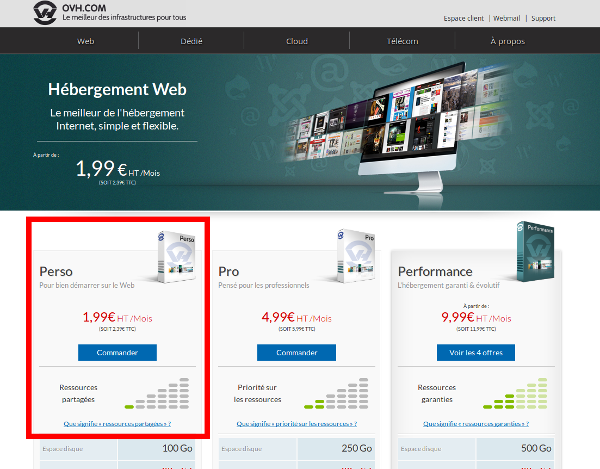
\includegraphics[scale=0.5]{img/0008.png}
\end{center}
\subsection{Comprendre les information envoyée par l'hébergeur}
\paragraph{}J'ai loué un hébergement mutualisé, que faire ensuite ?
\paragraph{}Vous avez loué un hébergement mutualisé et vous avez reçu un email avec des données étranges à l'intérieur... Nous allons apprendre à nous en servir !
\paragraph{}Voici un exemple de mail que vous recevrez :
\begin{center}
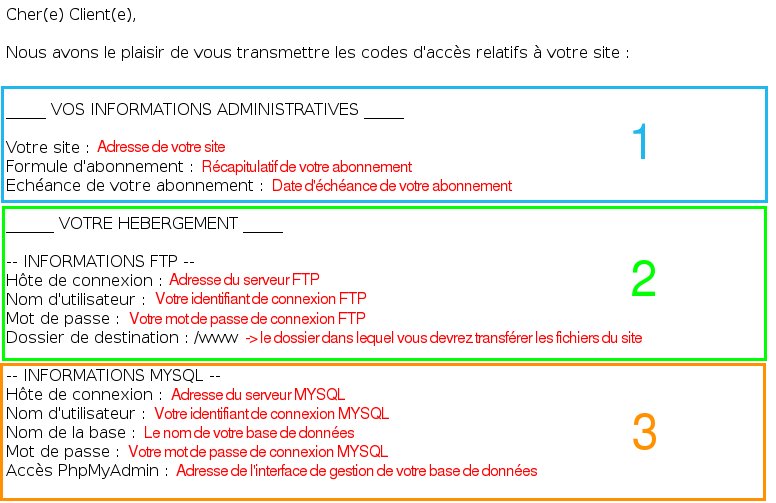
\includegraphics[scale=0.4]{img/0009.png}
\end{center}
\paragraph{}Décortiquons un peu ce mail.
\paragraph{}Première partie (encadrée en bleu) : Ce sont les données administratives. Elles rappellent simplement l'offre que vous avez choisi et la date d'échéance de celle-ci.
\paragraph{}Seconde partie (encadrée en vert) : Ce sont les données de l'espace de stockage de l'hébergement mutualisé, celui qui accueillera les fichiers de votre site Wordpress. Nous utiliserons ces données lors du transfert des fichiers de Wordpress.
\paragraph{}Troisième partie (encadrée en orange) : Ce sont les données de la base de données MYSQL que nous utiliserons lors de la procédure d'installation de Wordpress.
\newpage

\section{Transférer les fichiers de Wordpress sur un hébergement mutualisé}
\paragraph{}Nous avons, jusqu'à présent :
\begin{itemize}
\item Téléchargé Wordpress
\item Décompressé l'archive et préparé les fichiers du site
\item Choisi un hébergement mutualisé
\item Compris les données envoyées par notre hébergeur
\end{itemize}
\paragraph{}Nous sommes donc prêt à transférer les fichiers de Wordpress sur notre hébergement mutualisé !
\paragraph{}Enfin... presque...
\paragraph{}Le transfert des fichiers ne se fait pas par email ni par magie, il nous faut utiliser un logiciel spécifique et adapté à ce genre de tâche : un client FTP.

\subsection{Qu'est-ce qu'un client FTP?}
\paragraph{}Un client FTP est un logiciel qui, comme son nom l'indique, utilise le protocole FTP qui signifie Protocole de Transfert de Fichier (File Transfer Protocole en Anglais). Il permet donc, depuis un ordinateur, de copier des fichiers vers un autre ordinateur (un serveur par exemple...). Il permet aussi d'administrer un site web ou encore de supprimer ou modifier des fichiers sur cet ordinateur.
\begin{center}
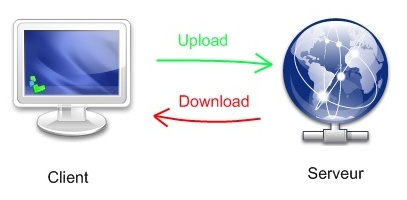
\includegraphics[scale=0.7]{img/0010.jpg}
\end{center}

\subsection{Un client FTP libre et gratuit: FileZilla}
\begin{center}

\includegraphics[scale=0.1]{img/0011.png}
\end{center}
\paragraph{}FileZilla est un client FTP puissant et complet. Il a l'avantage d'être libre et gratuit mais aussi multi-plateforme c'est à dire qu'il fonctionne aussi bien sous Windows que sous Linux et MacOs.
\paragraph{}Nous choisirons donc ce logiciel pour transférer les fichiers de 
Wordpress sur votre hébergement mutualisé.
\subsubsection{Installer FileZilla sous Microsoft Windows}
\paragraph{}Démarrez votre navigateur et rendez-vous à l'adresse suivante :
\paragraph{}http://filezilla-project.org/
\paragraph{}Une fois sur le site, cliquez sur « Download FileZilla Client » pour accéder à la page de téléchargement.
\begin{center}
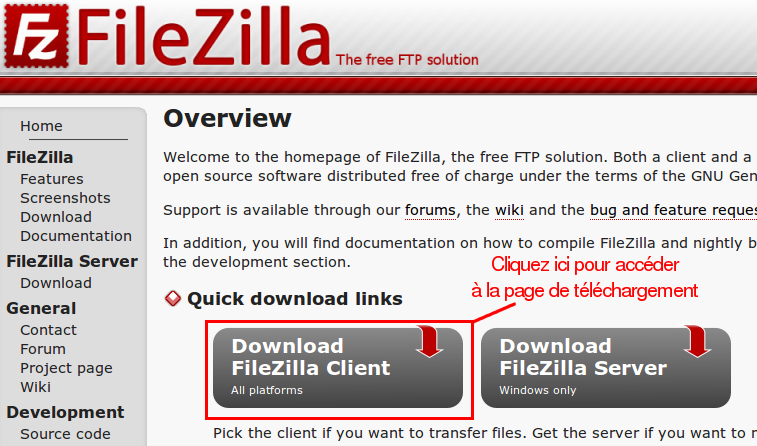
\includegraphics[scale=0.5]{img/0012.png}
\end{center}
\paragraph{}Une fois sur la page de téléchargement, cliquez sur « FileZilla\_x.x.x\_winXX-setup.exe » pour lancer le téléchargement du fichier d'installation de FileZilla
\begin{center}
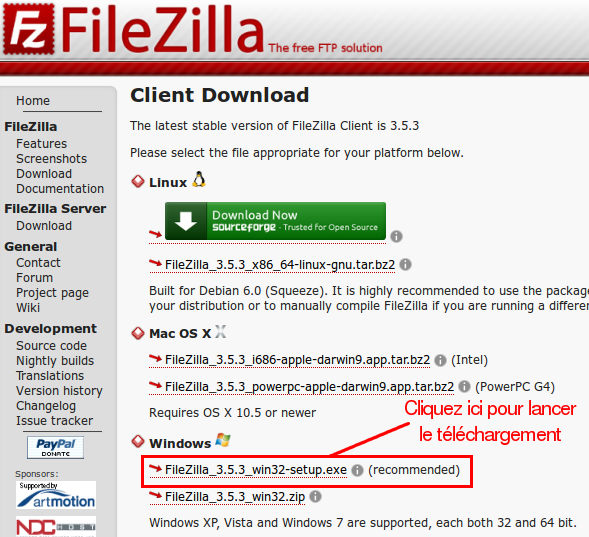
\includegraphics[scale=0.4]{img/0013.png}
\end{center}
\paragraph{}Dans la boîte de dialogue qui apparaît, sélectionnez « Enregistrer le fichier » (ou équivalent suivant votre navigateur) puis cliquez sur « Ok ».
\begin{center}
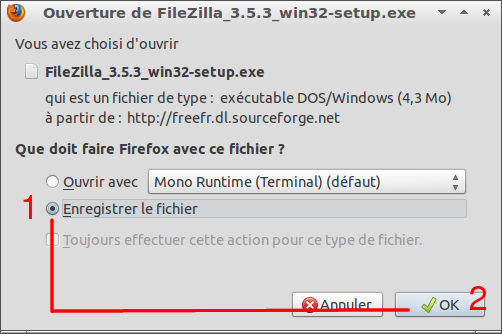
\includegraphics[scale=0.5]{img/0014.png}
\end{center}
\paragraph{}Le téléchargement se lance...
\begin{center}
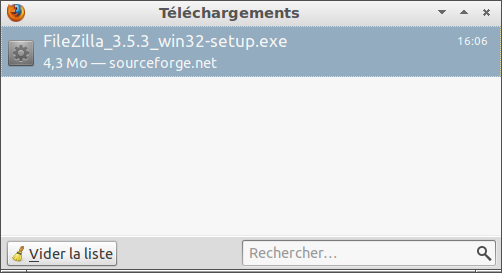
\includegraphics[scale=0.5]{img/0015.png}
\end{center}
\paragraph{}Rendez-vous dans le dossier Téléchargement situé dans votre répertoire personnel.
\paragraph{}Double-cliquez sur le fichier « FileZilla\_x.x.x\_winXX-setup.exe » pour commencer l'installation du logiciel.
\paragraph{}\textbf{Étape 1 : }Licence d'utilisation
\paragraph{}Acceptez la licence d'utilisation en cliquant sur « I Agree »
\begin{center}
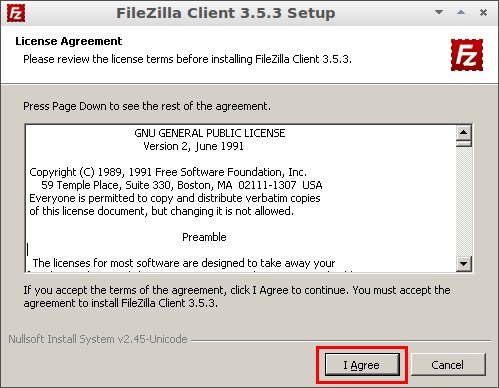
\includegraphics[scale=0.5]{img/0016.png}
\end{center}
\paragraph{}\textbf{Étape 2 : }Choix des options d'installation
\paragraph{}Sélectionnez qui aura accès à FileZilla sur votre ordinateur
\begin{itemize}
\item \textit{Anyone who use this computer (All users)} : Tous les utilisateurs pourront utiliser FileZilla
\item \textit{Only for me (Votre nom d'utilisateur)} : En cochant cette case, seul vous pourrez utilisez FileZilla
\end{itemize}
\begin{center}
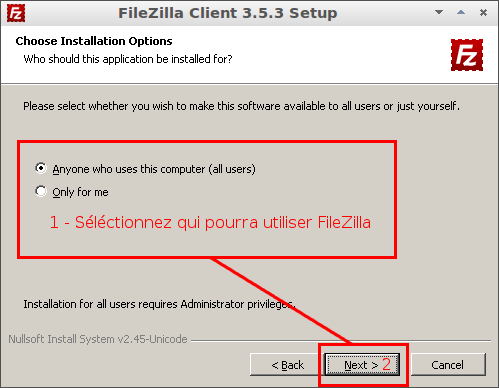
\includegraphics[scale=0.5]{img/0017.png}
\end{center}
\paragraph{}\textbf{Étape 3 : }Choix des composants
\paragraph{}Cochez la case « Desktop Icon » si vous souhaitez créer un raccourcis de FileZilla sur votre bureau. Cliquez ensuite sur « Next » pour poursuivre.
\begin{center}
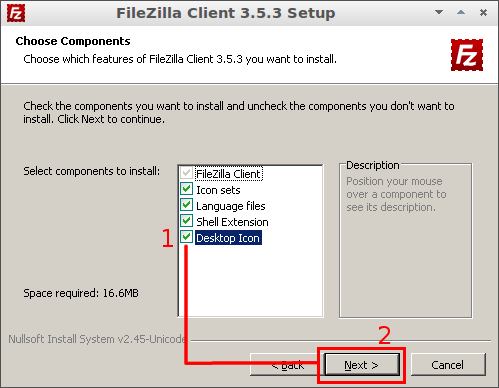
\includegraphics[scale=0.5]{img/0018.png}
\end{center}
\paragraph{}\textbf{Étape 4 : }Choix du répertoire d'installation
\paragraph{}Laissez le répertoire d'installation par défaut et cliquez « Next » pour poursuivre.
\begin{center}
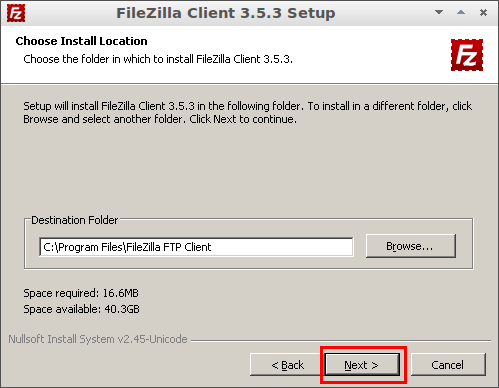
\includegraphics[scale=0.5]{img/0019.png}
\end{center}
\paragraph{}\textbf{Étape 5 : }Choix du dossier du menu Démarrer
\paragraph{}Laissez le choix par défaut puis cliquez sur «Install » pour lancer l'installation.
\begin{center}
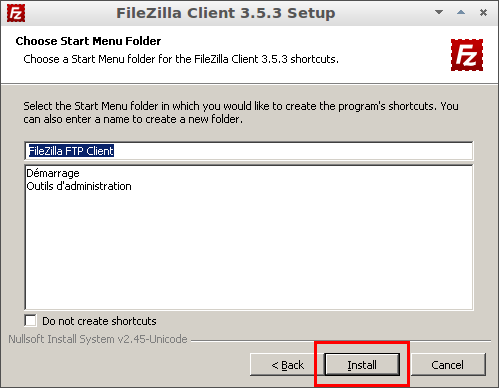
\includegraphics[scale=0.5]{img/0020.png}
\end{center}
\paragraph{}\textbf{Étape 6 : }L'installation est en cours...
\begin{center}
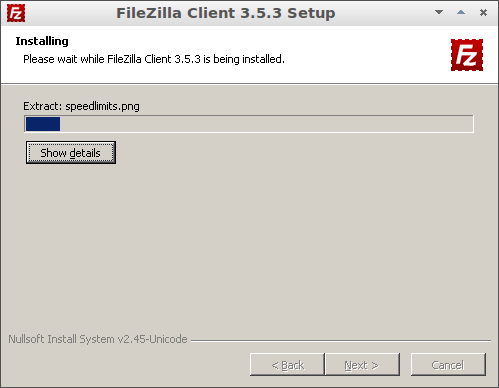
\includegraphics[scale=0.5]{img/0021.png}
\end{center}
\paragraph{}\textbf{Étape 7 : }L'installation est terminée
\paragraph{}L'installation est terminée, cochez la case « Start FileZilla nox » et cliquez sur « Finish » pour démarrer FileZilla.
\begin{center}
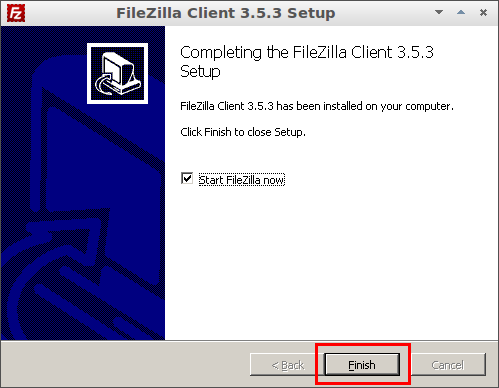
\includegraphics[scale=0.5]{img/0022.png}
\end{center}
\subsubsection{Installer FileZilla sous Linux Ubuntu}
\paragraph{}\textbf{Étape 1 : }Lancez la logithèque
\paragraph{}Lancez la logithèque
\begin{center}
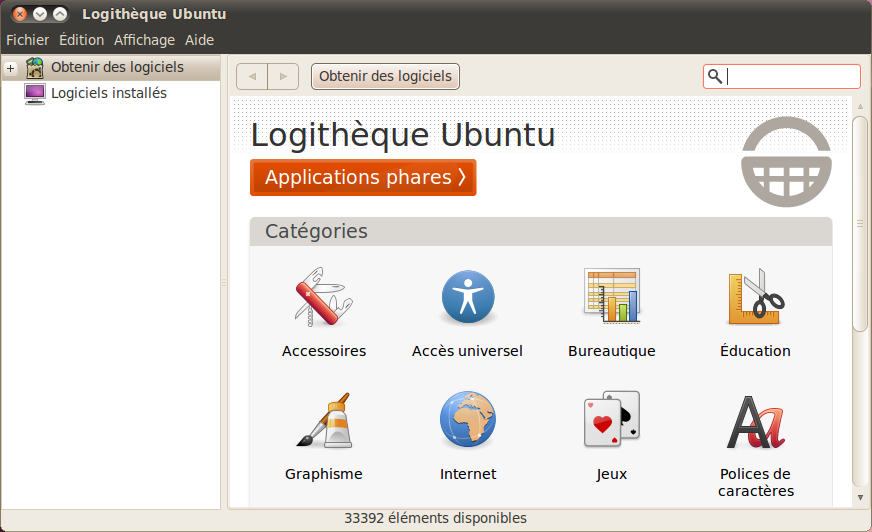
\includegraphics[scale=0.4]{img/0023.png}
\end{center}
\paragraph{}\textbf{Étape 2 : }Rechercher et installer FileZilla
\paragraph{}Recherchez Filezilla puis cliquez sur « Installer ».
\begin{center}
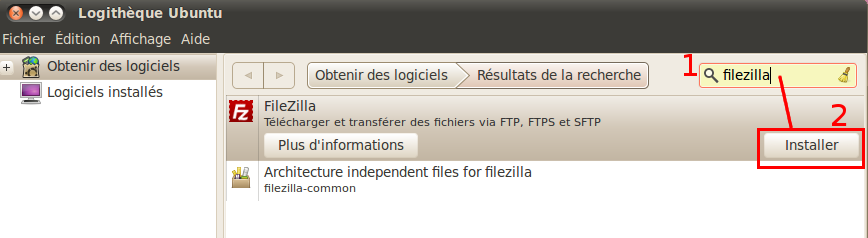
\includegraphics[scale=0.4]{img/0024.png}
\end{center}
\paragraph{}\textbf{Étape 3 : }Authentification
\paragraph{}Indiquez votre mot de passe super-utilisateur (ou root) puis cliquez sur « S'authentifier » pour lancer l'installation.
\begin{center}
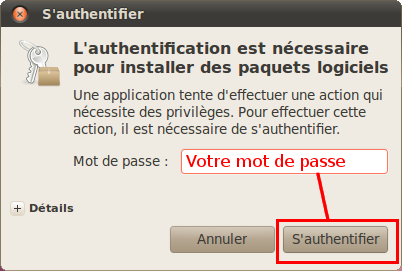
\includegraphics[scale=0.4]{img/0025.png}
\end{center}
\paragraph{}\textbf{Étape 4 : }Installation en cours...
\paragraph{}L'installation de FileZilla est en cours...
\begin{center}
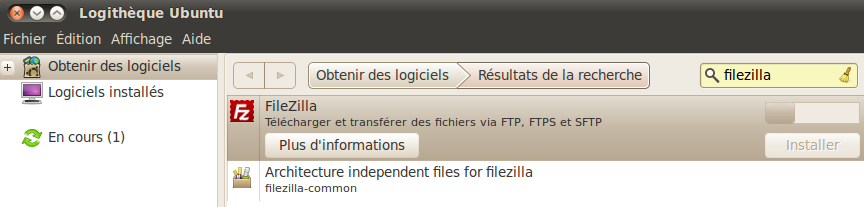
\includegraphics[scale=0.4]{img/0026.png}
\end{center}
\paragraph{}\textbf{Étape 5 : }Installation terminée
\paragraph{}L'installation est terminée !
\begin{center}
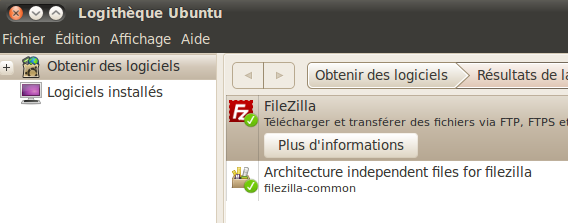
\includegraphics[scale=0.4]{img/0027.png}
\end{center}
\paragraph{}\textbf{Étape 6 : }Démarrer FileZilla
\paragraph{}Démarrez FileZilla en cliquant sur Applications > Internet > FileZilla.
\begin{center}
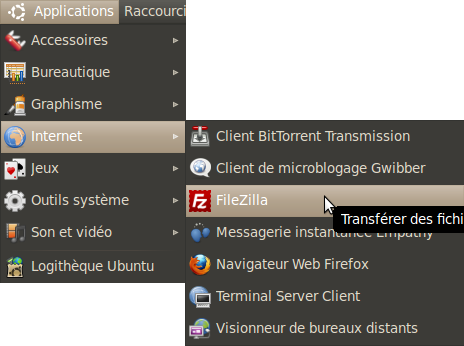
\includegraphics[scale=0.4]{img/0028.png}
\end{center}

\subsection{Tour d'horizon de FileZilla}
\subsubsection{Premier démarrage}
\paragraph{}Au premier lancement de FileZilla apparaît une boîte de dialogue vous indiquant notamment des liens vers de la documentation. Cliquez sur « Ok » pour fermer cette boîte de dialogue.
\begin{center}
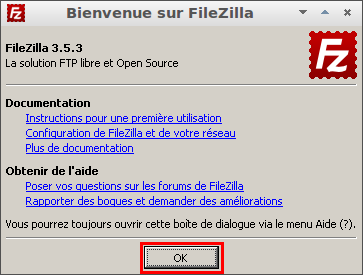
\includegraphics[scale=0.4]{img/0029.png}
\end{center}
\subsubsection{Décryptage de l'interface}
\paragraph{}Vous pouvez voir que la fenêtre principale de FileZilla est est divisée en plusieurs parties.
\begin{center}
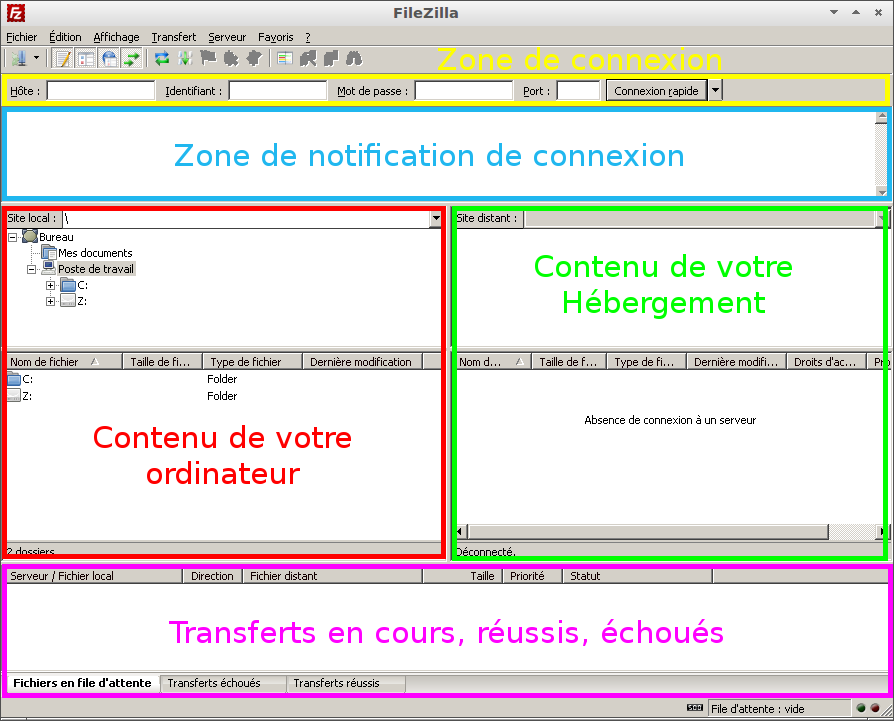
\includegraphics[scale=0.4]{img/0030.png}
\end{center}
\paragraph{}\textbf{Première partie (encadrée en jaune) :} La zone d'identification, c'est dans celle-ci que nous allons renseigner les informations de connexion pour accéder à l'espace de stockage que vous trouverez dans le mail que vous enverra votre hébergeur (voir ci-dessous).
\begin{center}
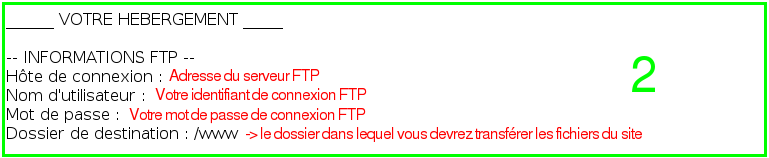
\includegraphics[scale=0.4]{img/0031.png}
\end{center}
\paragraph{}\textbf{Seconde partie (encadrée en bleu) :} La zone de notification de connexion. Vous y trouverez des informations concernant la connexion à votre hébergement (par exemple :connexion au serveur réussie ou échouée).
\paragraph{}\textbf{Troisième partie (encadrée en rouge) :} Le contenu de votre ordinateur. Affiche l'arborescence de votre ordinateur afin d'aller rechercher les fichiers à transférer sur votre hébergement.
\paragraph{}\textbf{Quatrième partie (encadrée en vert) :} Le contenu de votre hébergement (ou espace de stockage). Affiche l'arborescence de votre hébergement.
\paragraph{}\textbf{Cinquième partie (encadrée en rose) :} La zone de notification de transfert. Affiche les transferts en cours mais aussi leur statut (réussis ou échoués).

\subsection{Transférer les fichiers du site Wordpress sur l'hébergement Mutualisé}
\paragraph{}Nous sommes (enfin...) prêts à transférer les fichiers de Wordpress sur l'hébergement mutualisé.
\subsubsection{Connexion au serveur FTP}
\paragraph{}Si ce n'est pas déjà fait, démarrez FileZilla.
\paragraph{}Indiquez dans la zone de connexion les informations FTP envoyées par votre hébergeur.
\begin{center}

\includegraphics[scale=0.4]{img/0032.png}
\end{center}
\begin{enumerate}
\item Indiquez l'adresse du serveur FTP
\item Indiquez votre identifiant de connexion FTP
\item Indiquez votre mot de passe de connexion FTP
\item Indiquez le port FTP (sauf indication contraire de votre hébergeur, le port FTP est « 21 »)
\end{enumerate}
\paragraph{}Cliquez ensuite sur le bouton « Connexion rapide » pour vous connecter à votre hébergement mutualisé.
\paragraph{}Si tout s'est bien passé (pas de message d'erreur dans la zone de notification de connexion) vous devriez voir le contenu de votre hébergement à droite de l'écran (encadré en rouge ci-dessous).
\begin{center}
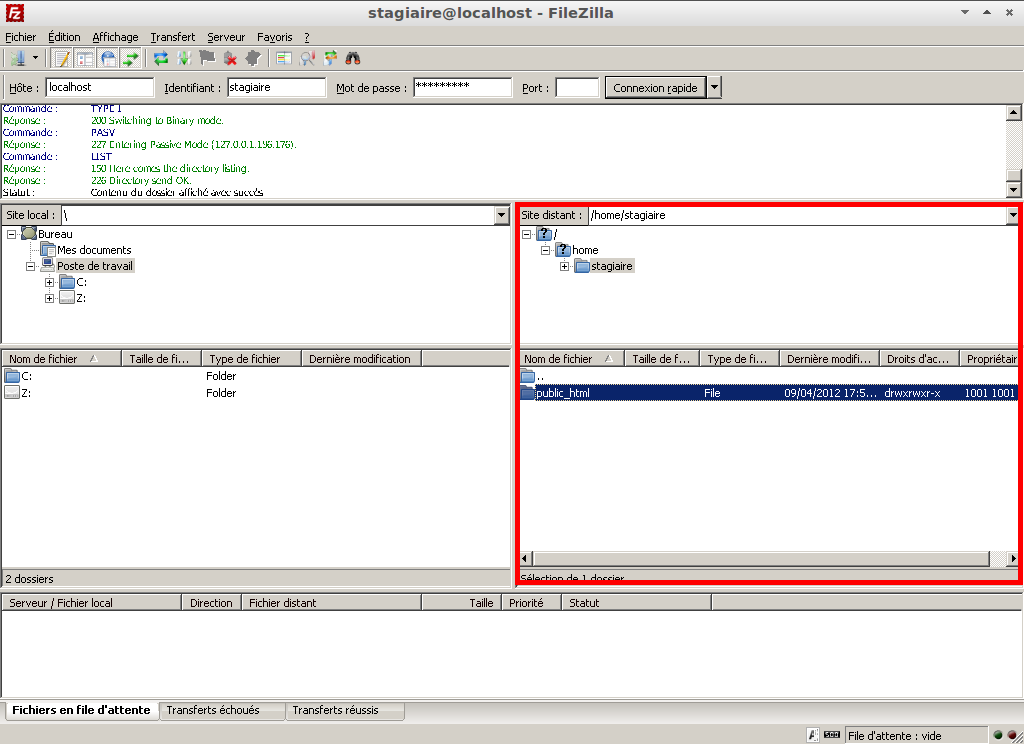
\includegraphics[scale=0.35]{img/0033.png}
\end{center}
\paragraph{}Pour le moment seul un répertoire (ici public\_html) s'y trouve. Selon votre hébergeur, ce répertoire peut s'appeler \textbf{www}, \textbf{public\_html} ou encore \textbf{web}. C'est dans ce répertoire que  vous devrez transférer les fichiers de Wordpress afin qu'ils soient visibles sur Internet.
\subsubsection{Transfert des fichiers}
\paragraph{}Double-cliquez sur le répertoire public\_html afin d'afficher son contenu.
\begin{center}
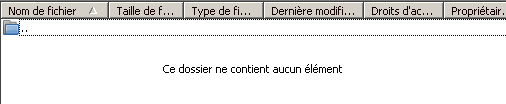
\includegraphics[scale=0.5]{img/0034.png}
\end{center}
\paragraph{}Pour le moment, il est vide...
\paragraph{}Dans la zone de contenu de votre ordinateur (encadrée en rouge ci-dessous) affichez les dossiers et fichiers de Wordpress que vous avez télécharger tout à l'heure (qui doivent normalement se situer dans le dossier Téléchargements de votre répertoire personnel).
\begin{center}
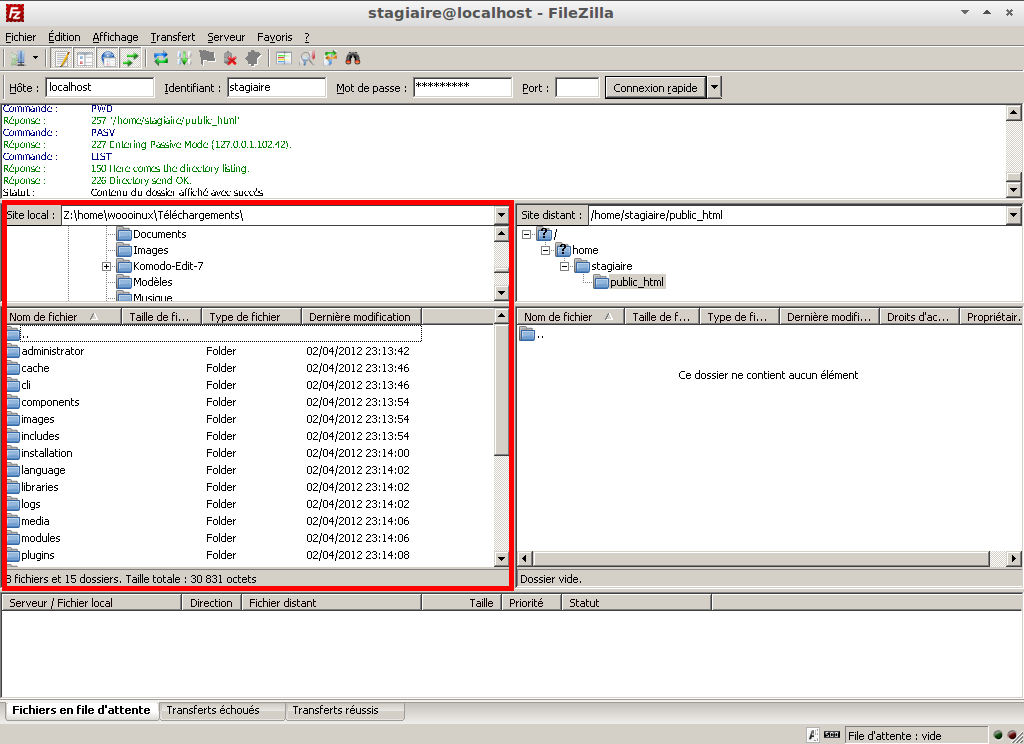
\includegraphics[scale=0.35]{img/0035.png}
\end{center}
\paragraph{}Sélectionnez tous les dossiers et fichiers puis faites un glisser-déposer vers le dossier public\_html de votre hébergement mutualisé.
\begin{center}
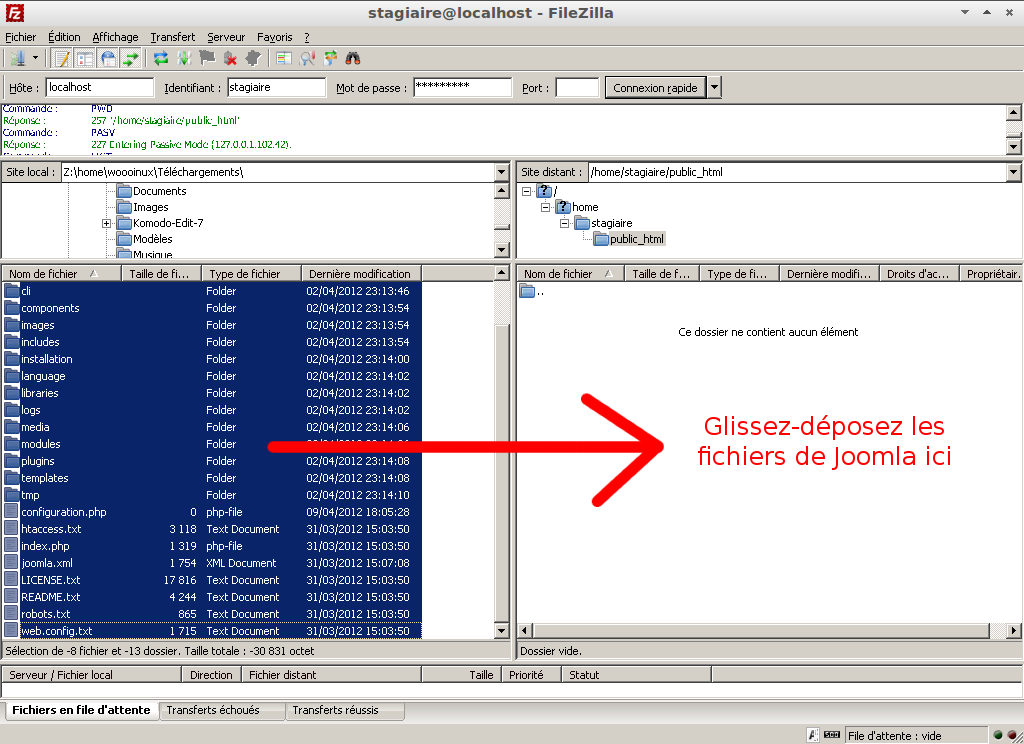
\includegraphics[scale=0.35]{img/0036.png}
\end{center}
\paragraph{}Le transfert des fichiers est en cours. Vous pouvez voir la progression et l'état du transfert dans la zone de notification des transferts (encadrée en rouge ci-dessous) et les fichiers apparaître dans le contenu de votre hébergement (encadré en vert ci-dessous).
\begin{center}
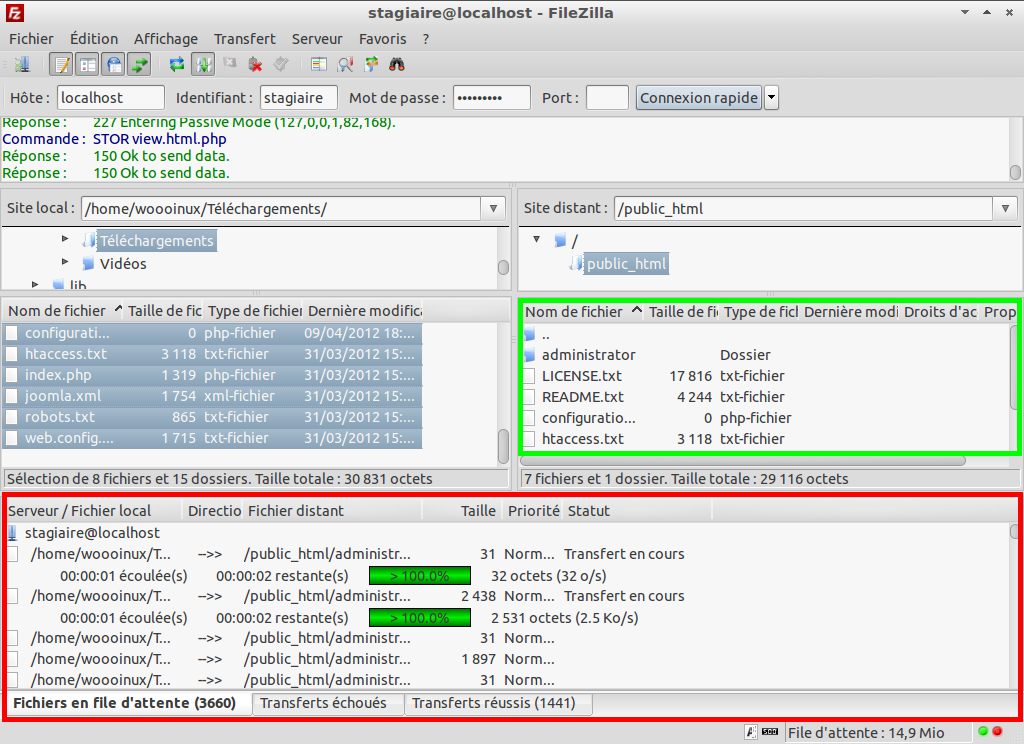
\includegraphics[scale=0.35]{img/0037.png}
\end{center}
\paragraph{}Si tout s'est bien passé (pas d'erreurs dans l'onglet Transferts échoués de la zone de notification des transferts) vous devriez voir tous les dossiers et fichiers de Wordpress dans le zone de contenu de votre hébergement (encadrée en rouge ci-dessous).
\begin{center}
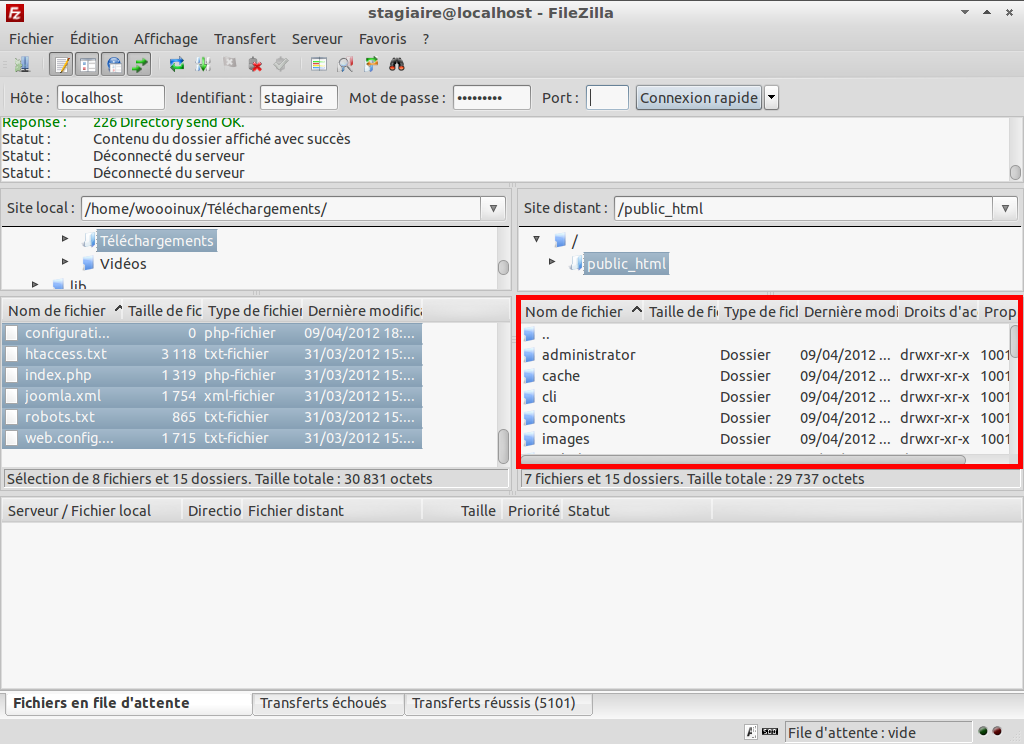
\includegraphics[scale=0.35]{img/0038.png}
\end{center}
\paragraph{}Vous pouvez maintenant quitter FileZilla.
\begin{center}
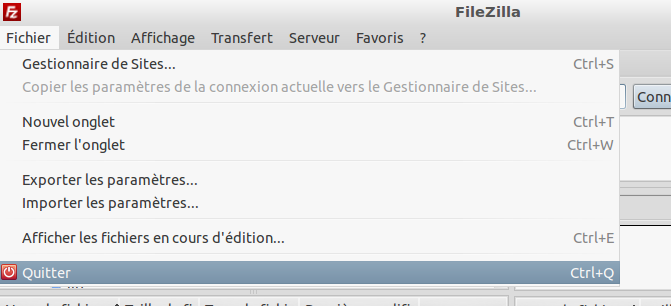
\includegraphics[scale=0.35]{img/0039.png}
\end{center}
\paragraph{}Nous avons maintenant terminé le transfert des fichiers Wordpress sur votre hébergement mutualisé, il en nous reste plus qu'à nous rendre sur le site afin de terminer l'installation.
\newpage

\section{Installer Wordpress}
\paragraph{}Accédez à votre site Wordpress en indiquant l'adresse fournie par votre hébergeur dans votre navigateur.
\paragraph{}Vous arrivez sur la page d'installation de Wordpress.
\paragraph{}\textbf{Étape 1 : }Avant propos
\paragraph{}Cette page récapitule toutes les informations dont vous aurez besoin pour mener l'installation jusqu'au bout. Si vous avez toutes ces informations, cliquez sur le bouton « C'est parti ! » pour lancer l'installation de Wordpress.
\begin{center}
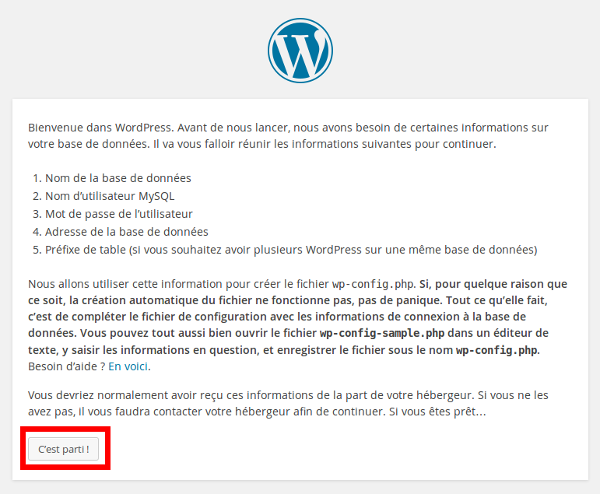
\includegraphics[scale=0.5]{img/0040.png}
\end{center}
\paragraph{}\textbf{Étape 2 : }Configuration de la base de données
\paragraph{}Cette étape est cruciale ! Vous devez indiquer les informations relatives à votre base de données afin que Wordpress puisse s'y connecter et y créer les tables dont il aura besoin.
\paragraph{}Par exemple voici comment remplir ce formulaire avec les informations que vous avez reçu lors de la formation (remplacer le « X » par votre numéro de stagiaire) :
\begin{center}
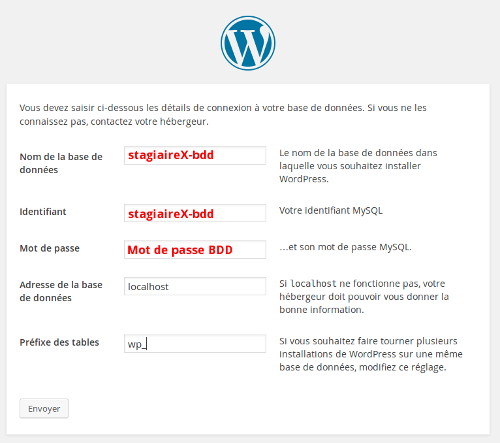
\includegraphics[scale=0.5]{img/0041.png}
\end{center}
\paragraph{}\textbf{Étape 3 : }Lancement de l'installation
\paragraph{}Si vous avez correctement renseigné les informations de connexion à votre base de données vous devriez arrivé sur une page vous disant que Wordpress est désormais capable de communiquer avec cette dernière. Cliquez sur le bouton « Lancer l 'installation » pour… lancer l'installation !
\begin{center}
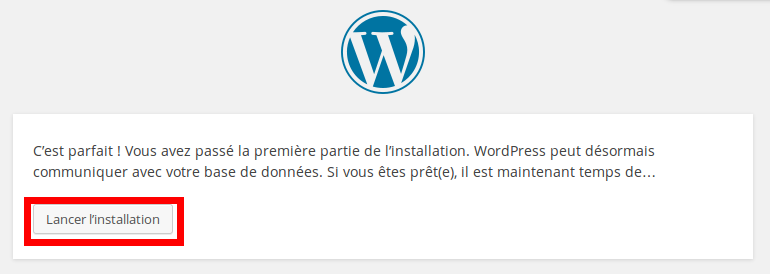
\includegraphics[scale=0.5]{img/0042.png}
\end{center}
\paragraph{}\textbf{Étape 4 : }Configuration de Wordpress
\paragraph{}Cette étape va vous permettre de configurer Wordpress. Vous allez donc donner un nom à votre site (le nom de votre structure par exemple), vous choisir un identifiant ainsi qu'un mot de passe pour accéder à l'administration et ainsi gérer votre site et enfin renseigné votre courriel.
\begin{center}
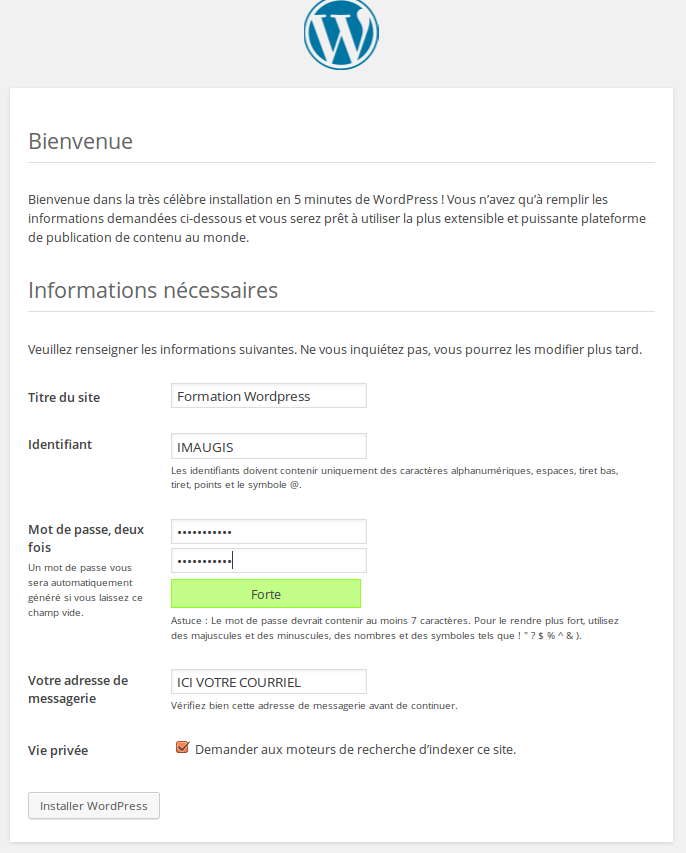
\includegraphics[scale=0.5]{img/0043.png}
\end{center}
\paragraph{}\textbf{Étape 5 : }Installation terminée
\paragraph{}Si l'installation de Wordpress s'est bien déroulée vous devriez voir apparaître une message de succès vous proposant aussi de vous connecter au back-office. Cliquez sur le bouton « Connexion » pour accéder au formulaire d'authentification :
\begin{center}
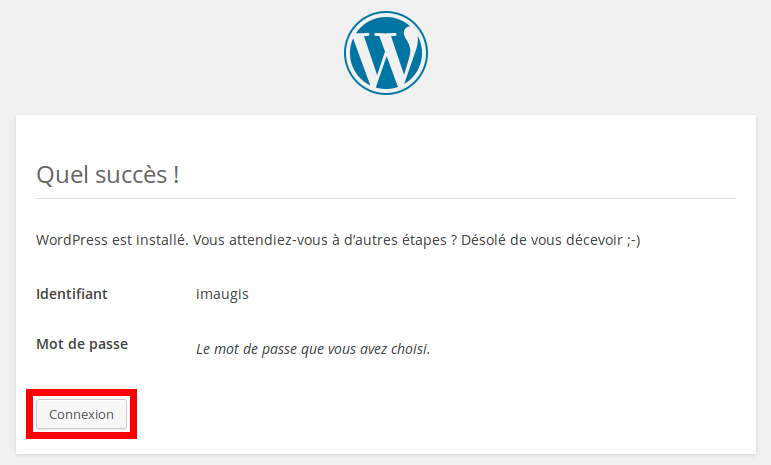
\includegraphics[scale=0.5]{img/0044.png}
\end{center}
\paragraph{}\textbf{Étape 6 : }Formulaire d'authentification
\paragraph{}Saisissez l'identifiant ainsi que le mot de passe choisis lors de l'installation (cf étape 4) et cliquez sur le bouton « Connexion ».
\begin{center}
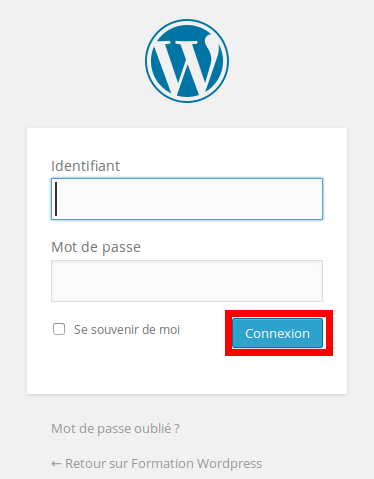
\includegraphics[scale=0.5]{img/0045.png}
\end{center}
\paragraph{}\textbf{Étape 7 : }Le Back-Office
\paragraph{}Si votre authentification s'est déroulée sans encombre vous devez arrivé sur le back-office de Wordpress. Félicitation ! L'installation de Wordpress est terminée !
\begin{center}
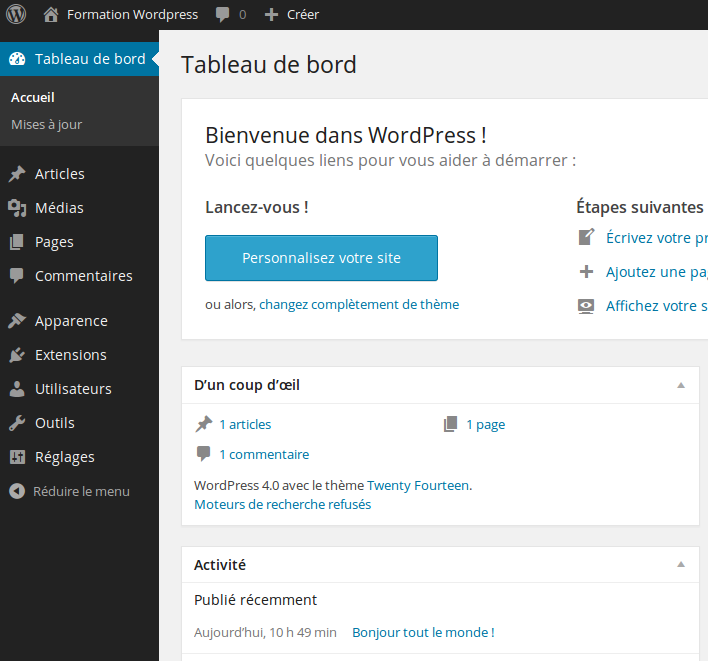
\includegraphics[scale=0.5]{img/0046.png}
\end{center}
\newpage

\part{Premiers pas avec Wordpress}
\newpage

\section{Tour d'horizon de Wordpress}
\paragraph{}Wordpress se décompose en deux partie principales : le front-office et le back-office.
\subsection{Le "Front-Office"}
\paragraph{}Le front-office est la partie site, la boutique, ce que voient les visiteurs qui viennent sur votre site.
\begin{center}
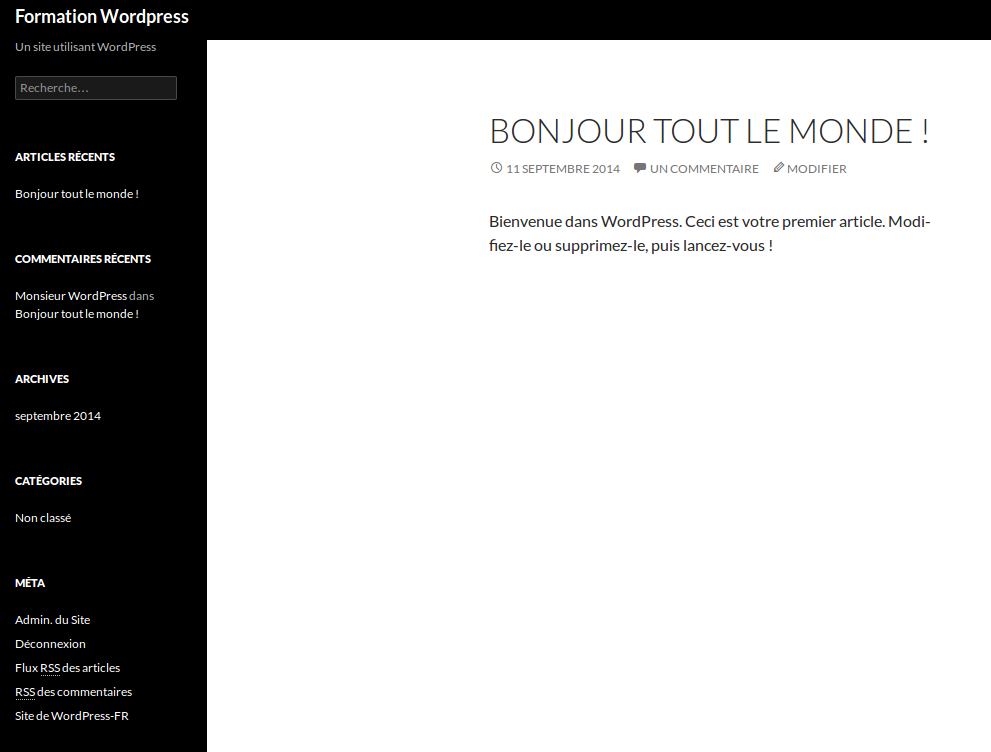
\includegraphics[scale=0.35]{img/0047.png}
\end{center}
\paragraph{}Le front-office affichera ce que vous aurez envie d'afficher c'est vous qui décidez !
\paragraph{}Par exemple : Vos articles, vos menus, vos galeries photos, vos vidéos, un forum de discussion, des sondages, etc...
\paragraph{}Pour accéder au front-office, il suffit d'entrer l'adresse de votre site (celle que vous aura communiquer votre hébergeur) dans la barre d'adresse de votre navigateur.
\paragraph{}Par exemple : http://www.monsite.com

\subsection{Le "Back-Office"}
\paragraph{}Le back-office est la partie administration. C'est l’arrière-boutique de votre site ; l'interface d’administration va permettre de créer et mettre à jour vos articles mais aussi de gérer tout votre site.
\begin{center}
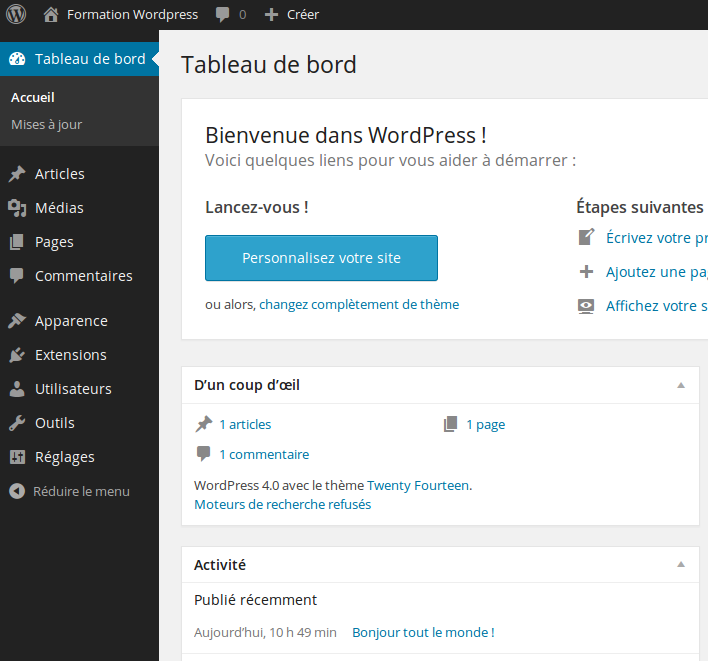
\includegraphics[scale=0.5]{img/0046.png}
\end{center}
\paragraph{}Comme expliqué plus haut, le back-office vous permettra de gérer le site :
\begin{itemize}
\item Ajouter, modifier, supprimer des articles
\item Créer des catégories pour organiser vos articles
\item Ajouter du contenu multimédia (images, sons)
\item Ajouter, modifier, supprimer des menus
\item Gérer les utilisateurs
\item D'ajouter des plugins, widgets et donc des fonctionnalités supplémentaires à Wordpress
\item De gérer le thème (design) du site
\item De mettre à jour Wordpress
\end{itemize}
\paragraph{}Pour accéder au back-office, il suffit d'entrer l'adresse de votre site suivi de « /wp-admin »
\paragraph{}Par exemple : http://www.monsite.com/wp-admin
\newpage

\section{Générer des permaliens plus propres}
\paragraph{}Un réglage important à effectuer après une installation fraîche de Wordpress et celle des « permaliens ».
\paragraph{}Les permaliens sont les adresses (URL) permanentes de vos articles, ainsi que des catégories, archives, et autres pages spéciales. Le permalien permet à un autre site de référer à l'un de vos articles, ou de pointer vers votre article depuis un courriel. L'adresse URL de chaque article est permanente, et ne doit jamais changer - d'où le terme de "perma"-lien.
\paragraph{}Par défaut, les permaliens sur Wordpress ne sont pas très lisibles. Par exemple, si on affiche le premier article présent sur votre site : Bonjour tout le monde. On voit une url un peu bizarre du genre :  http://www.monsite/com/?p=1.
\paragraph{}Nous allons donc rendre cette adresse (et toutes celle de vos futurs articles) plus lisible en affichant le titre de l'article dans l'url plutôt que l'identifiant en base de données de celui-ci.
\paragraph{}Pour se faire, rendez-vous dans le back-office et allez sur le menu « Réglages » puis « Permaliens »
\begin{center}
\includegraphics[scale=0.5]{img/0048.png}
\end{center}
\paragraph{}Sélectionnez « Nom de l'article » puis cliquez sur le bouton « Enregistrer les modifications ».
\begin{center}
\includegraphics[scale=0.4]{img/0049.png}
\end{center}
\paragraph{}Retournez sur le back-office affichez l'article « Bonjour tout le monde ». L'URL est maintenant http://www.monsite.com/bonjour-tout-le-monde ».
\newpage

\section{Effectuer les mises à jour de Wordpress}
\paragraph{}Effectuer les mises à jours que propose Wordpress et très important. En effet, les mises à jours peuvent corriger des bugs ou des failles de sécurité. Mais vous allez voir que faire ses mises à jour sous Wordpress est un jeu d'enfant.
\paragraph{}Avant toute chose vous allez déjà vous rendre compte que Wordpress vous avertit de la présence de mises à jour disponibles. En effet, lorsque vous vous connectez au back-office vous pourrez constater la présence de mises à jour en dessous de l'onglet « Tableau de bord » comme dans les exemples ci-dessous :
\begin{center}
\includegraphics[scale=0.5]{img/0050.png}
\end{center}
\begin{center}
\includegraphics[scale=0.5]{img/0051.png}
\end{center}
\paragraph{}Nous voyons très clairement dans cet exemple que 5 mises à jours sont disponibles.
\paragraph{}Par contre, une chose importante à savoir et qu'il existe 4 types de mises à jour :
\begin{itemize}
\item Les mises à jours du core (cœur) de Wordpress
\item Les mises à jours des extensions
\item Les mises à jour des thèmes
\item Les mises à jour des traductions
\end{itemize}
\paragraph{}Maintenant que vous savez tout, il n'y a plus qu'à effectuer les mises à jours (s'il y en a à faire bien évidemment…). Pour cela, rien de plus simple, cliquez sur le menu… « Mises à jour ».
\subsection{Mises à jour du core (cœur) de Wordpress}
\paragraph{}Dans le page des Mises à jour de Wordpress, en dessous du titre « Une nouvelle version de Wordpress est disponible » Cliquez sur le bouton « Mettre à jour ».
\begin{center}
\includegraphics[scale=0.35]{img/0052.png}
\end{center}
\paragraph{}Dans certains, cas une mise à jour peut vous demander de vous reconnecter.
\subsection{Mises à jour des extensions}
\paragraph{}Dans le page des Mises à jour de Wordpress (lorsque des mises à jour pour les extensions sont disponibles), cliquez sur « Tout sélectionner » en dessous du titre « Extensions » puis cliquez sur le bouton « Mettre à jour les extensions ».
\begin{center}
\includegraphics[scale=0.35]{img/0053.png}
\end{center}
\paragraph{}Une fois la mise à jour des extensions terminées cliquez sur le lien « Retourner aux mises à jour de Wordpress ».
\begin{center}
\includegraphics[scale=0.35]{img/0054.png}
\end{center}
\subsection{Mises à jour des thèmes}
\paragraph{}Dans le page des Mises à jour de Wordpress (lorsque des mises à jour pour les thèmes sont disponibles), cliquez sur « Tout sélectionner » en dessous du titre « Thèmes » puis cliquez sur le bouton « Mettre à jour les thèmes ».
\begin{center}
\includegraphics[scale=0.35]{img/0055.png}
\end{center}
\paragraph{}Une fois la mise à jour des thèmes terminées cliquez sur le lien « Retourner aux mises à jour de Wordpress ».
\begin{center}
\includegraphics[scale=0.35]{img/0056.png}
\end{center}
\subsection{Mises à jour des traductions}
\paragraph{}Dans le page des Mises à jour de Wordpress (lorsque des mises à jour pour les traductions sont disponibles), cliquez sur le bouton « Mise à jour des traductions ».
\begin{center}
\includegraphics[scale=0.35]{img/0057.png}
\end{center}
\paragraph{}Une fois la mise à jour des traductions terminées cliquez sur le lien « Retourner aux mises à jour de Wordpress ».
\begin{center}
\includegraphics[scale=0.35]{img/0058.png}
\end{center}
\paragraph{}Et voilà, vous avez installé, configuré, et mis a jour votre site Wordpress ! Maintenant vous pouvez :
\begin{itemize}
\item Ajouter vos contenus
\item Installer de nouveaux thèmes
\item Installer des extensions
\item et pleins de choses encore !
\end{itemize}
\newpage

\part{Les publications}
\newpage

\section{Les articles et les pages}
\paragraph{} \begin{center}\textit{La définition ci-dessous est extraite du cours "Propulsez votre site avec Wordpress" issu du site OpenClassrooms}\end{center}
\paragraph{} Sous WordPress, les contenus sont organisés en deux types : les articles et les pages. La différence entre les deux réside dans le type de contenu que vous allez placer à l’intérieur.
\begin{itemize}
\item \textbf{Un article} sera généralement un contenu d’actualité, c’est-à-dire qu’il prend sa plus grande valeur au moment de sa publication. C’est typiquement le type de contenu utilisé pour les publications d’un blog ou sur un fil d’actualité.
\item \textbf{Une page} aura au contraire un contenu à valeur constante dans le temps sans avoir besoin d’être mise à jour. On peut l’utiliser pour présenter une société, une personne ou bien pour parler d’un sujet de fond.
\end{itemize}
\paragraph{}Au niveau de la présentation, les articles peuvent être affichés en liste par ordre chronologique, puisque c’est ce qui fait leur sens, soit complètement soit avec un aperçu du contenu, tandis que les pages seront accessibles par un lien (le plus souvent dans le menu de navigation) vers leur contenu.
\subsection{Lister les articles et les pages}
\paragraph{}Pour lister les articles, cliquez sur le bouton « Articles » dans le menu de gauche de Wordpress.
\begin{center}
\includegraphics[scale=0.5]{img/0059.png}
\end{center}
\paragraph{}Vous obtiendrez alors la liste complète des articles présents sur votre site. Ces articles sont triés par défaut du plus récent au plus ancien.
\begin{center}
\includegraphics[scale=0.3]{img/0060.png}
\end{center}
\paragraph{}Pour lister les pages, cliquez sur le bouton « Pages » dans le menu de gauche de Wordpress.
\begin{center}
\includegraphics[scale=0.5]{img/0061.png}
\end{center}
\paragraph{}Vous obtiendrez alors la liste complète des pages présentes sur votre site. Ces pages sont triées par défaut de la plus récente à la plus ancienne.
\begin{center}
\includegraphics[scale=0.3]{img/0062.png}
\end{center}
\subsection{Ajouter, éditer ou supprimer un article ou une page}
\subsubsection{Ajouter un article ou une page}
\paragraph{}Pour ajouter un nouvel article ou une nouvelle page, cliquez sur... « Ajouter ».
\begin{center}
\begin{tabular}{cc}
\includegraphics[scale=0.35]{img/0063.png} &
\includegraphics[scale=0.4]{img/0065.png} \\
\end{tabular}
\end{center}
\paragraph{}Vous obtiendrez un formulaire pour écrire un nouvel article ou une nouvelle page.
\begin{center}
\includegraphics[scale=0.3]{img/0064.png}
\end{center}
\subsubsection{Éditer un article ou une page}
\paragraph{}Pour éditer un article ou une page, passez votre souris sur l'article ou la page en question afin de faire apparaître des options supplémentaires. Cliquez ensuite sur « Modifier ».
\begin{center}
\includegraphics[scale=0.35]{img/0066.png}
\end{center}
\paragraph{}Vous obtiendrez le formulaire pour éditer votre article ou votre page.
\begin{center}
\includegraphics[scale=0.35]{img/0067.png}
\end{center}
\subsubsection{Supprimer un article ou une page}
\paragraph{}Pour supprimer un article ou une page, passez votre souris sur l'article ou la page en question afin de faire apparaître des options supplémentaires. Cliquez ensuite sur « Mettre à la corbeille ».
\begin{center}
\includegraphics[scale=0.35]{img/0068.png}
\end{center}
\paragraph{}Il est important de préciser que l'action « Mettre à la corbeille » n'est pas irréversible. En effet, vous pouvez rétablir un article ou une page, que vous auriez supprimé accidentellement par exemple, dans la corbeille.
\paragraph{}Si votre corbeille contient au moins un élément, vous verrez alors apparaître « Corbeille » suivi du nombre d'éléments qu'elle contient entre parenthèses au-dessus de la liste de vos articles ou pages.
\paragraph{}Cliquez sur le bouton « Corbeille » pour afficher la liste des articles ou pages qu'elle contient.
\begin{center}
\includegraphics[scale=0.35]{img/0069.png}
\end{center}
\paragraph{}Passez votre souris sur un article ou une page pour faire apparaître des options supplémentaires et cliquez sur « Rétablir » si vous souhaitez... rétablir un article ou une page supprimés accidentellement ou bien cliquez sur « Supprimer définitivement » si vous souhaitez... supprimer définitivement un article ou une page.
\paragraph{}À noter que vous pouvez \textbf{supprimer définitivement} le contenu de la corbeille en cliquant sur le bouton « Vider la corbeille ».
\begin{center}
\includegraphics[scale=0.35]{img/0070.png}
\end{center}
\subsection{Le formatage d'un article ou d'une page}
\subsubsection{Les paragraphes}
\paragraph{} Le paragraphe est le formatage de texte par défaut dans l'éditeur de texte de Wordpress.
\begin{center}
\includegraphics[scale=0.35]{img/0071.png}
\end{center}
\subsubsection{Les niveaux de titres}
Pour créer un titre ou un sous-titre, sélectionnez le texte puis choisissez le niveau de titre souhaité dans la liste des styles de formatage.
\begin{center}
\includegraphics[scale=0.35]{img/0072.png}
\end{center}
\paragraph{}À noter que plus le chiffre est grand plus le titre est petit...
\subsubsection{Les listes à puces}
\paragraph{}Pour créer une liste à puces, sélectionnez les éléments de la liste puis cliquez sur le bouton « Liste à puces ».
\begin{center}
\includegraphics[scale=0.35]{img/0073.png}
\end{center}
\paragraph{}Vous obtiendrez une liste à puces.
\begin{center}
\includegraphics[scale=0.35]{img/0074.png}
\end{center}
\subsubsection{Les listes numérotées}
\paragraph{}Pour créer une liste numérotée, sélectionnez les éléments de la liste puis cliquez sur le bouton « Liste numérotée ».
\begin{center}
\includegraphics[scale=0.35]{img/0075.png}
\end{center}
\paragraph{}Vous obtiendrez une liste numérotée.
\begin{center}
\includegraphics[scale=0.35]{img/0076.png}
\end{center}
\subsubsection{Les liens internes}
\paragraph{}Un lien interne est un lien qui renvoie vers une autre page de votre site. Pour créer un lien interne sélectionnez le texte à transformer en lien puis cliquez sur le bouton « Insérer/modifier un lien ».
\begin{center}
\includegraphics[scale=0.35]{img/0077.png}
\end{center}
\paragraph{}Dans la fenêtre qui apparaît, cliquez sur le bouton « Ou alors, faites un lien vers l'un des contenus de votre site » pour faire apparaître la liste des articles et pages de votre site.
\paragraph{}Sélectionnez l'article ou la page souhaitée puis cliquez sur le bouton « Ajouter un lien ».
\begin{center}
\includegraphics[scale=0.35]{img/0078.png}
\end{center}
\paragraph{}Votre lien est créé.
\begin{center}
\includegraphics[scale=0.35]{img/0079.png}
\end{center}
\subsubsection{Les liens externes}
\paragraph{}Un lien externe est un lien qui renvoie vers un autre site Internet. Pour créer un lien externe sélectionnez le texte à transformer en lien puis cliquez sur le bouton « Insérer/modifier un lien ».
\begin{center}
\includegraphics[scale=0.35]{img/0077.png}
\end{center}
\paragraph{}Dans la fenêtre qui apparaît, indiquez l'adresse complète (avec http://) du site, cochez la case « Ouvrir le lien dans une nouvelle fenêtre/un nouvel onglet » puis cliquez sur le bouton « Ajouter un lien ».
\begin{center}
\includegraphics[scale=0.35]{img/0080.png}
\end{center}
\paragraph{}Votre lien est créé.
\begin{center}
\includegraphics[scale=0.35]{img/0079.png}
\end{center}
\subsubsection{Les liens de téléchargement}
\paragraph{}Il est parfois utile de donner la possibilité à vos visiteurs de pouvoir télécharger certains documents (comme un bulletin d'adhésion par exemple). Pour créer un lien de téléchargement cliquez sur le bouton « Ajouter un média ».
\begin{center}
\includegraphics[scale=0.35]{img/0081.png}
\end{center}
\paragraph{}Vous accédez au gestionnaire de médias.
\paragraph{}Là, vous avez deux cas de figure possible :
\paragraph{}\textbf{Cas 1 : }Le fichier que vous souhaitez mettre en téléchargement se trouve déjà dans votre gestionnaire de médias et donc vous n'avez qu'à le sélectionner puis cliquer sur le bouton « Insérer dans l'article ».
\begin{center}
\includegraphics[scale=0.3]{img/0082.png}
\end{center}
\paragraph{}\textbf{Cas 2 : }Le fichier que vous souhaitez mettre en téléchargement ne se trouve pas dans votre gestionnaire de médias et donc vous allez devoir l'envoyer.
\paragraph{}Pour cela, cliquez sur l'onglet « Envoyer des fichiers ».
\begin{center}
\includegraphics[scale=0.35]{img/0083.png}
\end{center}
\paragraph{}Cliquez ensuite sur le bouton « Choisir des fichiers » puis cherchez le fichier à mettre en téléchargement dans l'arborescence de votre ordinateur. Une fois le fichier trouvé, cliquez sur le bouton « Ouvrir » pour lancer l'envoie vers le gestionnaire de médias.
\begin{center}
\includegraphics[scale=0.35]{img/0084.png}
\end{center}
\paragraph{}À noter que la taille maximale d'un fichier que vous pouvez envoyer est indiquée en dessous du bouton « Choisir des fichiers ».
\paragraph{}Une fois l'envoie terminé, le fichier envoyé est automatiquement sélectionné, vous n'avez plus qu'à cliquer sur le bouton « Insérer dans l'article ».
\begin{center}
\includegraphics[scale=0.3]{img/0082.png}
\end{center}
\paragraph{}Le lien de téléchargement vers le fichier est créé cependant il prend, par défaut, le nom du fichier (sans l'extension). Il peut être judicieux de renommer le lien pour qu'il soit plus parlant. Pour cela, cliquez sur le lien. Vous devriez voir apparaître une infobulle en dessous de celui-ci. Cliquez sur le bouton « Modifier ».
\begin{center}
\includegraphics[scale=0.3]{img/0086.png}
\end{center}
\paragraph{}Dans la fenêtre qui apparaît, modifiez le champ « Texte du lien » puis cliquez sur le bouton « Mettre à jour » pour valider la modification.
\begin{center}
\includegraphics[scale=0.3]{img/0087.png}
\end{center}
\paragraph{}Et voilà, votre lien est désormais plus parlant ;)
\begin{center}
\includegraphics[scale=0.3]{img/0088.png}
\end{center}
\newpage

\section{La Taxonomie}
\subsection{Qu'est-ce que la taxonomie ?}
\paragraph{}La taxonomie est « un moyen de regrouper les choses entre elles ». Dans Wordpress, une taxonomie est un mécanisme de regroupement pour les articles. Il existe deux types de taxonomie dans Wordpress : Les catégories et les mots-clés (tags). La taxonomie ne s'applique qu'aux articles et non aux pages.
\subsection{Les catégories}
\paragraph{}Les catégories sont un premier moyen de regrouper vos articles par... catégories. Prenons l'exemple d'un site de recettes de cuisine. Les articles seront alors triés en trois catégories principales : Les entrées, les plats de résistance et les desserts. Afin de mieux organiser le contenu d'un site, il est également possible de créer des sous-catégories. Reprenons l'exemple du site de recettes de cuisine. Nous pouvons subdiviser les entrées en deux sous-catégories : Les entrées chaudes et les entrées froides. Ainsi l'internaute pourra afficher toutes les entrées (chaudes et froides) ou filtrer plus précisément (chaudes ou froides).
\subsubsection{Ajouter une nouvelle catégorie}
\paragraph{}Allez dans Articles > Catégories
\begin{center}
\includegraphics[scale=0.3]{img/0089.png}
\end{center}
\paragraph{}Indiquez le nom de la catégorie souhaitée puis cliquez sur le bouton « Ajouter une nouvelle catégorie ».
\begin{center}
\includegraphics[scale=0.3]{img/0090.png}
\end{center}
\paragraph{}Si tout s'est bien passé, la nouvelle catégorie apparaît dans la liste.
\begin{center}
\includegraphics[scale=0.3]{img/0091.png}
\end{center}
\subsubsection{Supprimer une catégorie}
\paragraph{}Pour supprimer une catégorie, passez votre souris sur la catégorie en question afin de faire apparaître des options supplémentaires puis cliquez tout simplement sur le bouton « Supprimer ».
\begin{center}
\includegraphics[scale=0.3]{img/0092.png}
\end{center}
\subsubsection{Ajouter une nouvelle sous-catégorie}
\paragraph{}Toujours dans Articles > Catégories, Indiquez le nom de la nouvelle sous-catégorie, sélectionnez la catégorie parente puis cliquez sur le bouton « Ajouter une nouvelle catégorie ».
\begin{center}
\includegraphics[scale=0.3]{img/0093.png}
\end{center}
\paragraph{}Si tout s'est bien passé, la nouvelle sous-catégorie apparaît dans la liste en dessous de sa catégorie parente.
\begin{center}
\includegraphics[scale=0.3]{img/0094.png}
\end{center}
\subsection{Les mots-clés}
\paragraph{}Les mots-clés (ou étiquettes ou tags) sont un autre moyen de regrouper vos articles. Par exemple, toujours dans l'exemple de recettes de cuisines, les mots-clés permettront de trier les recettes par aliment principal.
\subsubsection{Ajouter des mots-clés à un article}
\paragraph{}Pour ajouter un mot-clé à article allez dans l'édition de l'article en question. Sur la colonne de droite vous trouverez « Étiquettes ». Indiquez simplement le nom du mot-clé souhaité puis cliquez sur le bouton « Ajouter ».
\begin{center}
\includegraphics[scale=0.3]{img/0095.png}
\end{center}
\paragraph{}Si tout s'est bien passé, vous verrez le mot-clé apparaître en dessous du champ.
\begin{center}
\includegraphics[scale=0.3]{img/0096.png}
\end{center}
\subsubsection{Supprimer un mot-clé d'un article}
\paragraph{}Pour supprimer un mot-clé associé à un article, cliquez simplement sur la croix grise située à gauche du mot-clé à supprimer.
\begin{center}
\includegraphics[scale=0.3]{img/0097.png}
\end{center}
\newpage

\section{Les médias}
\subsection{L'image à la une}
\paragraph{}L'image à la une est l'image qui va représenter un article ou une page. Elle s'affiche, en fonction du thème choisi, en premier plan (sur la page d'accueil et sur les pages de catégories d'articles. Il ne faut donc pas la négliger.
\subsubsection{Ajouter une image à la une}
\paragraph{}Pour ajouter une image à la une dans un article ou une page allez dans l'édition de cette dernière puis, dans la colonne de droite, en descendant, vous trouverez un bloc « Image à la une ».
\paragraph{}Cliquez sur le bouton « Mettre une image à la une ».
\begin{center}
\includegraphics[scale=0.3]{img/0098.png}
\end{center}
\paragraph{}Dans le gestionnaire des médias, sélectionnez l'image souhaitée puis cliquez sur le bouton « Mettre une image à la une ». Si l'image souhaitée ne figure pas dans le gestionnaire des médias, cliquez sur l'onglet « Envoyer des fichiers » puis importez l'image depuis votre ordinateur.
\begin{center}
\includegraphics[scale=0.25]{img/0099.png}
\end{center}
\paragraph{}Si tout s'est bien passé vous devriez obtenir un aperçu de l'image à la une.
\begin{center}
\includegraphics[scale=0.3]{img/0100.png}
\end{center}
\subsubsection{Supprimer une image à la une}
\paragraph{}Pour supprimer une image à la une, allez dans l'édition de l'article ou la page concernée puis, dans le bloc « Image à la une », cliquez sur le bouton « Supprimer l'image à la une ».
\begin{center}
\includegraphics[scale=0.3]{img/0101.png}
\end{center}
\newpage
\subsection{Les images}
\paragraph{}En plus de l'image à la une, vous avez la possibilité d'agrémenter le corps de votre article ou de votre page d'images.
\subsubsection{Insérer une image dans le corps de l'article ou de la page}
\paragraph{}Pour insérer une image dans le corps d'un article ou d'une page, cliquez sur le bouton « Ajouter un média » situé au dessus de l'éditeur de texte.
\begin{center}
\includegraphics[scale=0.3]{img/0102.png}
\end{center}
\paragraph{}Dans le gestionnaire des médias, sélectionnez l'image souhaitée puis cliquez sur le bouton « Insérer dans l'article ». Si l'image souhaitée ne figure pas dans le gestionnaire des médias, cliquez sur l'onglet « Envoyer des fichiers » puis importez l'image depuis votre ordinateur.
\begin{center}
\includegraphics[scale=0.25]{img/0103.png}
\end{center}
\paragraph{}Si tout s'est bien passé, l'image sélectionnée est insérée dans le corps de l'article ou de la page.
\begin{center}
\includegraphics[scale=0.3]{img/0104.png}
\end{center}
\subsubsection{Redimensionner l'image}
\paragraph{}Cliquez sur l'image à redimensionner afin de faire apparaître les quatre poignées de redimensionnement.
\begin{center}
\includegraphics[scale=0.3]{img/0105.png}
\end{center}
\paragraph{}Cliquez sur l'une de ces poignées et tirez afin de redimensionner l'image à votre guise. À noter que les proportions seront toujours conservées.
\begin{center}
\includegraphics[scale=0.3]{img/0106.png}
\end{center}
\newpage
\subsubsection{L'alignement de l'image}
\paragraph{}Plusieurs options d'alignement s'offrent à vous :
\begin{itemize}
\item Centrer l'image
\item Aligner l'image à droite (avec contour de texte)
\item Aligner l'image à gauche (avec contour de texte)
\end{itemize}
\paragraph{Centrer l'image : }Pour centrer l'image, cliquez sur cette dernière afin de faire apparaître les option d'alignement.
\begin{center}
\includegraphics[scale=0.3]{img/0107.png}
\end{center}
\paragraph{}Cliquez sur le bouton « Centrer ».
\begin{center}
\includegraphics[scale=0.3]{img/0108.png}
\end{center}
\paragraph{}L'image est désormais centrée.
\begin{center}
\includegraphics[scale=0.3]{img/0109.png}
\end{center}
\paragraph{Aligner l'image à gauche : }Pour aligner l'image à gauche, cliquez sur cette dernière afin de faire apparaître les option d'alignement.
\begin{center}
\includegraphics[scale=0.3]{img/0107.png}
\end{center}
\paragraph{}À noter que pour faire passer le texte autour de l'image, ce dernier doit se trouver après l'image.
\paragraph{}Cliquez sur le bouton « Aligner à gauche ».
\begin{center}
\includegraphics[scale=0.3]{img/0110.png}
\end{center}
\paragraph{}L'image est désormais alignée à gauche et le texte passe autour.
\begin{center}
\includegraphics[scale=0.3]{img/0111.png}
\end{center}
\paragraph{Aligner l'image à droite : }Pour aligner l'image à droite, cliquez sur cette dernière afin de faire apparaître les option d'alignement.
\begin{center}
\includegraphics[scale=0.3]{img/0107.png}
\end{center}
\paragraph{}À noter que pour faire passer le texte autour de l'image, ce dernier doit se trouver après l'image.
\paragraph{}Cliquez sur le bouton « Aligner à droite ».
\begin{center}
\includegraphics[scale=0.3]{img/0112.png}
\end{center}
\paragraph{}L'image est désormais alignée à droite et le texte passe autour.
\begin{center}
\includegraphics[scale=0.3]{img/0113.png}
\end{center}
\newpage
\subsection{Insérer une galerie d'images}
\subsubsection{Créer une galerie d'images}
\paragraph{}Pour insérer une galerie d'image dans un article ou une page, cliquez sur le bouton « Ajouter un média » situé au dessus de l'éditeur de texte.
\begin{center}
\includegraphics[scale=0.3]{img/0102.png}
\end{center}
\paragraph{}Cliquez ensuite sur le bouton « Créer une galerie ».
\begin{center}
\includegraphics[scale=0.3]{img/0114.png}
\end{center}
\paragraph{}Sélectionnez les images souhaitées puis cliquez sur le bouton « Créer une nouvelle galerie ». Si les images souhaitées ne se trouvent pas dans le gestionnaire de médias, importez-les depuis votre ordinateur en cliquant sur l'onglet « Envoyer des fichiers ».
\begin{center}
\includegraphics[scale=0.25]{img/0115.png}
\end{center}
\paragraph{}Une fois la galerie créée, vous arrivez sur une page vous permettant de paramétrer la galerie avant de l'insérer sur l'article ou la page et notamment :
\begin{enumerate}
\item D'ajouter de nouvelles images
\item De modifier l'ordre des images en les faisant glisser / déposer là où vous le souhaitez
\item De supprimer des images de la galerie en cliquant sur la croix en haut à droite d'une miniature
\item De modifier le nombre de colonne (3 par défaut)
\end{enumerate}
\paragraph{}Une fois votre galerie paramétrée, cliquez sur le bouton « Insérer la galerie ».
\begin{center}
\includegraphics[scale=0.25]{img/0116.png}
\end{center}
\paragraph{}La galerie d'images est désormais insérée dans le corps de votre article ou de votre page.
\begin{center}
\includegraphics[scale=0.3]{img/0117.png}
\end{center}
\newpage
\subsubsection{Modifier une galerie d'images}
\paragraph{}Pour modifier une galerie d'images, cliquez une fois dessus afin de faire apparaître les options de modification et cliquez sur le bouton « Modifier ».
\begin{center}
\includegraphics[scale=0.3]{img/0118.png}
\end{center}
\paragraph{}Vous accédez à une page vous permettant de modifier la galerie et notamment :
\begin{enumerate}
\item D'ajouter de nouvelles images
\item De modifier l'ordre des images en les faisant glisser / déposer là où vous le souhaitez
\item De supprimer des images de la galerie en cliquant sur la croix en haut à droite d'une miniature
\item De modifier le nombre de colonne (3 par défaut)
\end{enumerate}
\paragraph{}Une fois votre galerie modifiée, cliquez sur le bouton « Mettre à jour la galerie ».
\begin{center}
\includegraphics[scale=0.25]{img/0116.png}
\end{center}
\newpage
\subsubsection{Supprimer une galerie d'images}
\paragraph{}Pour supprimer une galerie d'image, cliques une fois dessus pour faire apparaître les options de modification et cliquez sur le bouton « Supprimer ».
\begin{center}
\includegraphics[scale=0.3]{img/0119.png}
\end{center}
\newpage
\subsection{Insérer un fichier audio}
\paragraph{}Pour insérer un fichier audio dans un article ou une page, cliquez sur le bouton « Ajouter un média » situé au dessus de l'éditeur de texte.
\begin{center}
\includegraphics[scale=0.3]{img/0102.png}
\end{center}
\paragraph{}Dans le gestionnaire des médias, sélectionnez le fichier audio souhaité puis cliquez sur le bouton « Insérer dans l'article ». Si le fichier audio souhaité ne figure pas dans le gestionnaire des médias, cliquez sur l'onglet « Envoyer des fichiers » puis importez le depuis votre ordinateur.
\begin{center}
\includegraphics[scale=0.25]{img/0120.png}
\end{center}
\paragraph{}Si tout s'est bien passé, un lecteur audio est inséré dans le corps de l'article ou de la page.
\begin{center}
\includegraphics[scale=0.3]{img/0121.png}
\end{center}
\paragraph{}Et voilà, c'est aussi simple que ça !
\newpage
\subsection{Insérer une liste de lecture audio}
\paragraph{}Pour insérer une liste de lecture audio dans un article ou une page, cliquez sur le bouton « Ajouter un média » situé au dessus de l'éditeur de texte.
\begin{center}
\includegraphics[scale=0.3]{img/0102.png}
\end{center}
\paragraph{}Dans le gestionnaire des médias, cliquez sur le bouton « Créer une liste de lecture audio ».
\begin{center}
\includegraphics[scale=0.3]{img/0122.png}
\end{center}
\paragraph{}Sélectionnez les fichiers audio souhaités puis cliquez sur le bouton « Créer une nouvelle liste de lecture audio ». Si les fichiers audio souhaités ne figurent pas dans le gestionnaire des médias, cliquez sur l'onglet « Envoyer des fichiers » puis importez les depuis votre ordinateur.
\begin{center}
\includegraphics[scale=0.25]{img/0123.png}
\end{center}
\newpage
\paragraph{}Vous accédez à une page vous permettant de paramétrer la liste et notamment :
\begin{enumerate}
\item D'ajouter de nouveaux fichiers audio
\item De modifier l'ordre des fichiers audio en les faisant glisser / déposer là où vous le souhaitez
\item De supprimer des fichiers audio de la liste en cliquant sur la croix en haut à droite d'une miniature
\end{enumerate}
\paragraph{}Une fois votre liste paramétrée, cliquez sur le bouton « Insérer une liste de lecture audio ».
\begin{center}
\includegraphics[scale=0.25]{img/0124.png}
\end{center}
\paragraph{}Si tout s'est bien passé, un lecteur audio est inséré dans le corps de l'article ou de la page.
\begin{center}
\includegraphics[scale=0.3]{img/0125.png}
\end{center}
\newpage
\subsection{Insérer une vidéo}
\paragraph{}Pour insérer un fichier vidéo dans un article ou une page, cliquez sur le bouton « Ajouter un média » situé au dessus de l'éditeur de texte.
\begin{center}
\includegraphics[scale=0.3]{img/0102.png}
\end{center}
\paragraph{}Dans le gestionnaire des médias, sélectionnez le fichier vidéo souhaité puis cliquez sur le bouton « Insérer dans l'article ». Si le fichier vidéo souhaité ne figure pas dans le gestionnaire des médias, cliquez sur l'onglet « Envoyer des fichiers » puis importez le depuis votre ordinateur.
\begin{center}
\includegraphics[scale=0.25]{img/0126.png}
\end{center}
\paragraph{}Si tout s'est bien passé, un lecteur vidéo est inséré dans le corps de l'article ou de la page.
\begin{center}
\includegraphics[scale=0.3]{img/0127.png}
\end{center}
\newpage
\subsection{Insérer une liste de lecture vidéo}
\paragraph{}Pour insérer une liste de lecture vidéo dans un article ou une page, cliquez sur le bouton « Ajouter un média » situé au dessus de l'éditeur de texte.
\begin{center}
\includegraphics[scale=0.3]{img/0102.png}
\end{center}
\paragraph{}Dans le gestionnaire des médias, cliquez sur le bouton « Créer une liste de lecture vidéo ».
\begin{center}
\includegraphics[scale=0.3]{img/0128.png}
\end{center}
\paragraph{}Sélectionnez les fichiers vidéo souhaités puis cliquez sur le bouton « Créer une nouvelle liste de lecture vidéo ». Si les fichiers vidéo souhaités ne figurent pas dans le gestionnaire des médias, cliquez sur l'onglet « Envoyer des fichiers » puis importez les depuis votre ordinateur.
\begin{center}
\includegraphics[scale=0.25]{img/0129.png}
\end{center}
\newpage
\paragraph{}Vous accédez à une page vous permettant de paramétrer la liste et notamment :
\begin{enumerate}
\item D'ajouter de nouveaux fichiers vidéo
\item De modifier l'ordre des fichiers vidéo en les faisant glisser / déposer là où vous le souhaitez
\item De supprimer des fichiers vidéo de la liste en cliquant sur la croix en haut à droite d'une miniature
\end{enumerate}
\paragraph{}Une fois votre liste paramétrée, cliquez sur le bouton « Insérer une liste de lecture vidéo ».
\begin{center}
\includegraphics[scale=0.25]{img/0130.png}
\end{center}
\paragraph{}Si tout s'est bien passé, un lecteur vidéo est inséré dans le corps de l'article ou de la page.
\begin{center}
\includegraphics[scale=0.3]{img/0131.png}
\end{center}
\newpage
\subsection{Insérer une vidéo depuis une plate-forme externe}
\subsubsection{Insérer une vidéo depuis Youtube}
\paragraph{}Rendez-vous sur Youtube et copiez l'adresse complète de la page affichant la vidéo que vous souhaitez intégrer dans votre article ou votre page.
\begin{center}
\includegraphics[scale=0.3]{img/0132.png}
\end{center}
\paragraph{}Revenez sur l'édition de votre article ou de votre page et cliquez sur le bouton « Ajouter un média » situé au dessus de l'éditeur de texte.
\begin{center}
\includegraphics[scale=0.3]{img/0102.png}
\end{center}
\paragraph{}Cliquez ensuite sur le bouton « Insérer à partir d'une adresse web ».
\begin{center}
\includegraphics[scale=0.3]{img/0133.png}
\end{center}
\newpage
\paragraph{}Supprimez « http:// » dans le champs qui apparaît puis collez l'adresse que vous avez copié précédemment.
\begin{center}
\includegraphics[scale=0.3]{img/0134.png}
\end{center}
\paragraph{}Vous devriez voir apparaître un lecteur. Cliquez enfin sur le bouton « Insérer dans l'article ».
\begin{center}
\includegraphics[scale=0.25]{img/0135.png}
\end{center}
\paragraph{}Si tout s'est bien passé, un lecteur est inséré dans le corps de l'article ou de la page.
\begin{center}
\includegraphics[scale=0.3]{img/0136.png}
\end{center}
\newpage
\subsubsection{Insérer une vidéo depuis Dailymotion}
\paragraph{}Rendez-vous sur Dailymotion et copiez l'adresse complète de la page affichant la vidéo que vous souhaitez intégrer dans votre article ou votre page.
\begin{center}
\includegraphics[scale=0.3]{img/0137.png}
\end{center}
\paragraph{}Revenez sur l'édition de votre article ou de votre page et cliquez sur le bouton « Ajouter un média » situé au dessus de l'éditeur de texte.
\begin{center}
\includegraphics[scale=0.3]{img/0102.png}
\end{center}
\paragraph{}Cliquez ensuite sur le bouton « Insérer à partir d'une adresse web ».
\begin{center}
\includegraphics[scale=0.3]{img/0133.png}
\end{center}
\newpage
\paragraph{}Supprimez « http:// » dans le champs qui apparaît puis collez l'adresse que vous avez copié précédemment.
\begin{center}
\includegraphics[scale=0.3]{img/0134.png}
\end{center}
\paragraph{}Vous devriez voir apparaître un lecteur. Cliquez enfin sur le bouton « Insérer dans l'article ».
\begin{center}
\includegraphics[scale=0.25]{img/0138.png}
\end{center}
\paragraph{}Si tout s'est bien passé, un lecteur est inséré dans le corps de l'article ou de la page.
\begin{center}
\includegraphics[scale=0.3]{img/0139.png}
\end{center}
\newpage
\subsubsection{Insérer une vidéo depuis Vimeo}
\paragraph{}Rendez-vous sur Vimeo et copiez l'adresse complète de la page affichant la vidéo que vous souhaitez intégrer dans votre article ou votre page.
\begin{center}
\includegraphics[scale=0.3]{img/0140.png}
\end{center}
\paragraph{}Revenez sur l'édition de votre article ou de votre page et cliquez sur le bouton « Ajouter un média » situé au dessus de l'éditeur de texte.
\begin{center}
\includegraphics[scale=0.3]{img/0102.png}
\end{center}
\paragraph{}Cliquez ensuite sur le bouton « Insérer à partir d'une adresse web ».
\begin{center}
\includegraphics[scale=0.3]{img/0133.png}
\end{center}
\newpage
\paragraph{}Supprimez « http:// » dans le champs qui apparaît puis collez l'adresse que vous avez copié précédemment.
\begin{center}
\includegraphics[scale=0.3]{img/0134.png}
\end{center}
\paragraph{}Vous devriez voir apparaître un lecteur. Cliquez enfin sur le bouton « Insérer dans l'article ».
\begin{center}
\includegraphics[scale=0.25]{img/0141.png}
\end{center}
\paragraph{}Si tout s'est bien passé, un lecteur est inséré dans le corps de l'article ou de la page.
\begin{center}
\includegraphics[scale=0.3]{img/0142.png}
\end{center}
\newpage

\part{La gestion des menus}
\newpage
\section{Créer un nouveau menu}
\subsubsection{Créer un nouveau menu}
\paragraph{}Pour créer un nouveau menu, rendez-vous dans Apparence > Menus.
\begin{center}
\includegraphics[scale=0.3]{img/0143.png}
\end{center}
\paragraph{}Cliquez sur le bouton « Créez un nouveau menu ».
\begin{center}
\includegraphics[scale=0.3]{img/0144.png}
\end{center}
\paragraph{}Renseignez le nom de votre menu (par exemple : menu principal) puis cliquez sur le bouton « Créer le menu ».
\begin{center}
\includegraphics[scale=0.3]{img/0145.png}
\end{center}
\paragraph{}Indiquez l'emplacement du thème dans lequel vous souhaitez placer votre menu (noms d'emplacement différents suivant les thèmes) puis cliquez sur le bouton « Enregistrer le menu ».
\begin{center}
\includegraphics[scale=0.3]{img/0146.png}
\end{center}
\paragraph{}Vous êtes désormais prêt à insérer des éléments dans votre menu.
\newpage
\subsection{Insérer une page dans le menu}
\paragraph{}Dans l'onglet « Pages », cliquez sur le bouton « Afficher tout » pour afficher toutes les pages de votre site.
\begin{center}
\includegraphics[scale=0.3]{img/0147.png}
\end{center}
\paragraph{}Sélectionnez la ou les pages à insérer dans le menu en cochant la ou les cases correspondantes puis cliquez sur le bouton « Ajouter au menu ».
\begin{center}
\includegraphics[scale=0.3]{img/0148.png}
\end{center}
\subsection{Insérer un lien personnalisé dans le menu}
\paragraph{}Dans l'onglet « Liens personnalisés », renseignez l'adresse complète (avec http://) du site vers lequel vous voulez créer un lien, renseignez ensuite le nom que prendra cet élément dans le menu puis cliquez enfin sur le bouton « Ajouter au menu ».
\begin{center}
\includegraphics[scale=0.3]{img/0149.png}
\end{center}
\subsection{Insérer une catégorie dans le menu}
\paragraph{}Dans l'onglet « Catégories », cliquez sur le bouton « Afficher tout » pour afficher toutes les catégories de votre site.
\begin{center}
\includegraphics[scale=0.3]{img/0150.png}
\end{center}
\paragraph{}Sélectionnez la ou les catégories à insérer dans le menu en cochant la ou les cases correspondantes puis cliquez sur le bouton « Ajouter au menu ».
\begin{center}
\includegraphics[scale=0.3]{img/0151.png}
\end{center}
\subsection{Créer un menu déroulant}
\paragraph{}Pour apprendre à créer un menu déroulant nous allons reprendre l'exemple de notre site de recettes de cuisine qui nous a été utile pour la gestion des catégories. Nous allons donc faire en sorte d'avoir un élément parent (les entrées) qui permettra d'afficher la liste des articles catégorisés « Les entrées » et donc obtenir la liste de toutes les recettes d'entrées (froides et chaudes). Puis nous allons y ajouter deux éléments enfants : Les entrées froides (qui permettra d'obtenir la liste des recettes d'entrées froides), et les entrées chaudes (qui permettra d'obtenir la liste des recettes des entrées chaudes).
\paragraph{}Commencez par ajouter l'élément parent (si ce n'est pas déjà fait).
\paragraph{}Dans l'onglet « Catégories », cliquez sur le bouton « Afficher tout » pour afficher toutes les catégories de votre site.
\begin{center}
\includegraphics[scale=0.3]{img/0150.png}
\end{center}
\paragraph{}Sélectionnez la catégorie « Les entrées » puis cliquez sur le bouton « Ajouter au menu ».
\begin{center}
\includegraphics[scale=0.3]{img/0151.png}
\end{center}
\paragraph{}Toujours dans l'onglet « Catégories », cliquez sur le bouton « Afficher tout » pour afficher toutes les catégories de votre site.
\begin{center}
\includegraphics[scale=0.3]{img/0150.png}
\end{center}
\paragraph{}Sélectionnez les catégories « Les entrées froides » et « Les entrées chaudes » puis cliquez sur le bouton « Ajouter au menu ».
\begin{center}
\includegraphics[scale=0.3]{img/0152.png}
\end{center}
\paragraph{}À ce stade, vous devez avoir les catégories « Les entrées froides » et « Les entrées chaudes » en dessous de la catégorie « Les entrées ».
\begin{center}
\includegraphics[scale=0.3]{img/0153.png}
\end{center}
\paragraph{}Pour créer un menu déroulant, les éléments enfants doivent se situer en dessous de l'élément parent (ce qui est déjà le cas) et être décalés d'un cran vers la droite (ce qui n'est pas encore le cas à ce stade).
\paragraph{}Pour décaler un élément, cliquez sur ce dernier sans relâcher puis décalez-le d'un cran vers la droite. Vous verrez des pointillés apparaître pour vous aider à visualiser le futur positionnement de votre élément. Quand ce dernier vous semble bon il suffit de relâcher le clic.
\begin{center}
\includegraphics[scale=0.3]{img/0154.png}
\end{center}
\paragraph{}Répétez l'opération pour chaque éléments enfants et voilà, votre menu déroulant est créé.
\begin{center}
\includegraphics[scale=0.3]{img/0155.png}
\end{center}
\newpage

\part{La gestion des utilisateurs}
\newpage
\section{Les rôles}
\paragraph{}Le système de Rôles a pour objectif de donner au propriétaire du blog la possibilité de contrôler et de déterminer ce que chaque utilisateur peut ou ne peut pas voir sur le blog. Un propriétaire de blog doit gérer et autoriser les accès à plusieurs fonctions comme la rédaction et l'édition de billets, la création de pages, la gestion des liens, la création des catégories, la modération des commentaires, la gestion des extensions, la gestion des thèmes, et la gestion des autres utilisateurs. Cet outil offre au propriétaire du blog, la possibilité d'attribuer un rôle à un utilisateur. 
\paragraph{}La notion de Rôles a été introduite à compter de la Version 2.0 de WordPress qui est livré 'de base' avec 5 rôles pré-définis : Administrateur, Éditeur, Auteur, Contributeur, and Abonné. Chaque rôle est pensé pour remplir plusieurs tâches appelées Permissions. Il y a trente Permissions dont la publication des billets, la modération des commentaires, et la gestion des utilisateurs. Les Permissions sont pré-déterminées pour chaque Rôle.
\paragraph{}Voici un aperçu des rôles et de leurs permissions dans Wordpress :
\begin{center}
\includegraphics[scale=0.5]{img/0156.png}
\end{center}
\newpage
\section{Ajouter, modifier ou supprimer un utilisateur}
\subsection{Ajouter un nouvel utilisateur}
\paragraph{}Pour ajouter un nouvel utilisateur rendez-vous dans Utilisateurs > Ajouter.
\begin{center}
\includegraphics[scale=0.3]{img/0157.png}
\end{center}
\paragraph{}Vous accédez à un formulaire vous demandant plusieurs renseignements :
\begin{itemize}
\item Identifiant (obligatoire) : C'est l'identifiant qui servira pour se connecter
\item E-mail (obligatoire) : L'adresse email du nouvel utilisateur
\item Prénom (optionnel) : Le prénom du nouvel utilisateur
\item Nom (optionnel) : Le nom du nouvel utilisateur
\item Site web (optionnel) : Si le nouvel utilisateur possède un site web, vous pouvez en indiquer l'adresse complète (avec http://) ici
\item Mot de passe (automatique) : Wordpress va générer automatiquement un mot de passe pour le nouvel utilisateur. Ce dernier aura la possibilité de le modifier via un lien de réinitialisation de mot de passe qui lui sera envoyé dès que vous aurez validez l'ajout.
\item Rôle (obligatoire) : Sélectionnez le rôle qu'aura le nouvel utilisateur (Abonné par défaut)
\end{itemize}
\paragraph{}Une fois tous les champs correctement renseignés, cliquez sur le bouton « Ajouter un utilisateur ».
\begin{center}
\includegraphics[scale=0.3]{img/0158.png}
\end{center}
\paragraph{}Le nouvel utilisateur recevra un courriel l'informant de la création de son compte et lui permettant de réinitialiser son mot de passe.
\subsection{Modifier un utilisateur}
\paragraph{}Pour modifier un utilisateur rendez-vous dans Utilisateurs > Tous les utilisateurs pour accéder à la liste des utilisateurs.
\begin{center}
\includegraphics[scale=0.3]{img/0159.png}
\end{center}
\paragraph{}Passez votre souris au dessus de l'utilisateur à modifier pour faire apparaître des options supplémentaires puis cliquez sur le bouton « Modifier ».
\begin{center}
\includegraphics[scale=0.3]{img/0160.png}
\end{center}
\subsection{Supprimer un utilisateur}
\paragraph{}Pour supprimer un utilisateur rendez-vous dans Utilisateurs > Tous les utilisateurs pour accéder à la liste des utilisateurs.
\begin{center}
\includegraphics[scale=0.3]{img/0159.png}
\end{center}
\paragraph{}Passez votre souris au dessus de l'utilisateur à supprimer pour faire apparaître des options supplémentaires puis cliquez sur le bouton « Supprimer ».
\begin{center}
\includegraphics[scale=0.3]{img/0161.png}
\end{center}
\paragraph{}Wordpress vous demande ce qu'il doit faire des éventuels publications de cet utilisateur. Deux choix s'offrent à vous :
\begin{itemize}
\item Supprimer tout le contenu de cet utilisateur
\item Attribuer tout le contenu de cet utilisateur à un autre utilisateur
\end{itemize}
\paragraph{}Je vous laisse le choix ;)
\paragraph{}Une fois votre choix effectué, cliquez sur le bouton « Confirmer la suppression » pour supprimer \textbf{définitivement} l'utilisateur.
\begin{center}
\includegraphics[scale=0.3]{img/0162.png}
\end{center}
\newpage

\part{La gestion des extensions}
\newpage

\section{Qu'est-ce qu'une extension ?}
\paragraph{}Une extension (ou plugin) est un programme qui va permettre d'ajouter une fonctionnalité supplémentaire à Wordpress. Par exemple, vous aurez la possibilité d'ajouter un gestionnaire d'événements, un système de newsletter, une boutique en ligne, et bien d'autres fonctionnalités encore...
\paragraph{}Par défaut, Wordpress a déjà installé deux extensions :
\begin{itemize}
\item \textbf{Askimet} est une extension anti-spam basique et très populaire pour lutter contre les commentaires indésirables sur votre blog.
\item \textbf{Hello Dolly} n'est pas vraiment une extension d'une utilité formidable. En effet, cette dernière va simplement afficher une phrase au hasard de la chanson « Hello Dolly » de Louis Armstrong dans le back-office de Wordpress.
\end{itemize}
\subsection{Activer une extension}
\paragraph{}Rendez-vous dans Extensions > Extensions installées pour afficher la liste des extensions présentes sur votre site.
\begin{center}
\includegraphics[scale=0.3]{img/0163.png}
\end{center}
\paragraph{}Vous pouvez voir l'existence d'Askimet et d'Hello Dolly. Cependant, ces extensions sont certes, installées sur votre site mais sont inactives par défaut.
\begin{center}
\includegraphics[scale=0.3]{img/0164.png}
\end{center}
\paragraph{}Pour activer une extension, cliquez sur le bouton « Activer ».
\begin{center}
\includegraphics[scale=0.3]{img/0165.png}
\end{center}
\paragraph{}Vous pouvez constater désormais qu'il est visuellement facile de faire la différence entre une extension activée ou non :
\begin{itemize}
\item Le terme « Activer » est remplacé par « Désactiver »
\item Le nom de l'extension apparaît désormais en gras
\item Une bordure bleue apparaît à gauche de l'extension
\end{itemize}
\begin{center}
\includegraphics[scale=0.3]{img/0166.png}
\end{center}
\subsection{Désactiver une extension}
\paragraph{}Pour désactiver une extension, cliquez sur le bouton « Désactiver ».
\subsection{Supprimer une extension}
\paragraph{}Pour supprimer une extension, il faut déjà commencer par la désactiver (voir un peu plus haut), puis cliquez sur le bouton « Supprimer ».
\begin{center}
\includegraphics[scale=0.3]{img/0167.png}
\end{center}
\paragraph{}Confirmez la suppression en cliquant sur le bouton « Oui, supprimer ces fichiers ».
\begin{center}
\includegraphics[scale=0.3]{img/0168.png}
\end{center}
\paragraph{}Si tout s'est bien passé, vous obtenez un message de confirmation de la bonne suppression de l'extension.
\begin{center}
\includegraphics[scale=0.3]{img/0169.png}
\end{center}
\newpage
\section{Installer de nouvelles extensions}
\paragraph{}Pour installer une nouvelle extension, rendez-vous dans Extensions > Ajouter.
\begin{center}
\includegraphics[scale=0.3]{img/0170.png}
\end{center}
\paragraph{}Renseignez le nom de l'extension à installer dans le champ de recherche puis validez en tapant sur la touche « Entrée ».
\begin{center}
\includegraphics[scale=0.3]{img/0171.png}
\end{center}
\paragraph{}Dans la page de résultat de la recherche qui suit, cliquez sur le bouton « Installer maintenant » pour lancer l'installation de l'extension.
\begin{center}
\includegraphics[scale=0.3]{img/0172.png}
\end{center}
\paragraph{}Une fois l'installation terminée, cliquez sur le bouton « Activer l'extension » pour la rendre opérationnelle.
\begin{center}
\includegraphics[scale=0.3]{img/0173.png}
\end{center}
\paragraph{}L'extension est désormais présente sur votre site et opérationnelle.
\begin{center}
\includegraphics[scale=0.3]{img/0174.png}
\end{center}
\newpage
\section{Connecter son site sur les réseaux sociaux avec Hupso Share Buttons}
\paragraph{}Hupso Share Buttons est une extension qui va permettre à vos visiteurs de partager vos articles ou vos pages à travers leurs réseaux sociaux favoris. Solution idéale et surtout gratuite pour communiquer à plus grande échelle.
\subsection{Installer Hupso Share Buttons}
\paragraph{}Recherchez et installez l'extension « Hupso Share Buttons ».
\begin{center}
\includegraphics[scale=0.3]{img/0175.png}
\end{center}
\paragraph{}N'oubliez pas d'activer l'extension.
\subsection{Paramétrer Hupso Share Buttons}
\paragraph{}Rendez-vous dans Réglages > Hupso Share Buttons.
\begin{center}
\includegraphics[scale=0.3]{img/0176.png}
\end{center}
\paragraph{}Sur cette page vous pourrez paramétrer :
\begin{itemize}
\item Le type de boutons de partage
\item La taille de la barre d'outils
\item La langue du terme « Partager »
\item La liste des réseaux sociaux
\item La position des boutons de partage
\item Les types de contenus sur lesquels vous souhaitez voir apparaître les boutons de partage
\end{itemize}
\begin{center}
\includegraphics[scale=0.3]{img/0177.png}
\end{center}
\paragraph{}Nous ne nous attarderons pas sur les autres paramétrages possibles.
\paragraph{}Une fois les paramétrages terminés, cliquez sur le bouton « Sauvegarder les paramètres ».
\paragraph{}Côté front-office vous verrez désormais apparaître des boutons qui permettront à vos visiteurs de partager vos articles et pages sur leurs réseaux sociaux favoris.
\begin{center}
\includegraphics[scale=0.3]{img/0178.png}
\end{center}
\newpage
\section{Ajouter un formulaire de contact grâce Formidables Forms}
\subsection{Installer Formidable Forms}
\paragraph{}Recherchez et installez l'extension « Formidable Forms ».
\begin{center}
\includegraphics[scale=0.3]{img/0179.png}
\end{center}
\paragraph{}N'oubliez pas d'activer l'extension.
\subsection{Créer un formulaire de contact}
\paragraph{}Rendez-vous dans Formidable > Formulaires.
\begin{center}
\includegraphics[scale=0.3]{img/0180.png}
\end{center}
\paragraph{}Cliquez sur le bouton « Modèles ».
\begin{center}
\includegraphics[scale=0.3]{img/0181.png}
\end{center}
\paragraph{}Passez votre souris sur le modèle « Contact Us » afin de faire apparaître des options supplémentaires puis cliquez sur le bouton « Créer un formulaire à partir du modèle ».
\begin{center}
\includegraphics[scale=0.3]{img/0182.png}
\end{center}
\paragraph{}Vous accédez au formulaire de création d'un... formulaire.
\paragraph{}Commencez par traduire le titre du formulaire puis la description de ce dernier.
\begin{center}
\includegraphics[scale=0.3]{img/0183.png}
\end{center}
\paragraph{}Traduisez les noms des champs qui sont, malheureusement en anglais par défaut.
\begin{center}
\includegraphics[scale=0.3]{img/0184.png}
\end{center}
\paragraph{}Vous avez la possibilité de supprimer des champs qui vous sembleraient inutiles en cliquant sur le bouton « Supprimer le champ » correspondant.
\begin{center}
\includegraphics[scale=0.3]{img/0185.png}
\end{center}
\paragraph{}Une fois ces réglages terminés, cliquez sur le bouton « Créer » pour valider la construction du formulaire.
\begin{center}
\includegraphics[scale=0.3]{img/0186.png}
\end{center}
\paragraph{}Vous accédez maintenant au paramétrage du formulaire.
\paragraph{Dans l'onglet « Général »} Traduisez le texte du bouton envoyer, le message de validation de soumission du formulaire puis cliquez sur le bouton « Mise à jour ».
\begin{center}
\includegraphics[scale=0.3]{img/0187.png}
\end{center}
\paragraph{Dans l'onglet « Actions du formulaire »} Cliquez sur « Email Notification » pour déplier les options puis modifiez si besoin le champ « à » qui comprend « [admin\_email] » ce qui correspond à l'adresse email créée lors de l'installation de Wordpress. Si cette adresse ne convient pas, supprimez « [admin\_email] » puis renseignez une adresse email à la place. Renseignez le sujet puis cliquez enfin sur le bouton « Mise à jour ».
\begin{center}
\includegraphics[scale=0.3]{img/0188.png}
\end{center}
\subsection{Insérer le formulaire de contact sur une page}
\paragraph{}Rendez-vous dans Pages > Ajouter puis créez une page ayant comme titre, par exemple, « Nous contacter ».
\paragraph{}Cliquez sur le bouton « Formidable » situé au dessus de l'éditeur de texte.
\begin{center}
\includegraphics[scale=0.3]{img/0189.png}
\end{center}
\paragraph{}Sélectionnez le formulaire de contact dans la liste déroulante puis cliquez sur le bouton « Insérer dans l'article ».
\begin{center}
\includegraphics[scale=0.25]{img/0190.png}
\end{center}
\paragraph{}Le formulaire s'insère dans le corps de la page sous la forme d'un shortcode.
\begin{center}
\includegraphics[scale=0.3]{img/0191.png}
\end{center}
\paragraph{}Ajouter la page « Nous contacter » à votre menu principal puis allez la visiter. Vous devriez voir un joli formulaire de contact.
\begin{center}
\includegraphics[scale=0.3]{img/0192.png}
\end{center}
\newpage
\section{Ajouter un gestionnaire d'événements avec The Events Calendar}
\subsection{Installer The Events Calendar}
\paragraph{}Recherchez et installez l'extension « The Events Calendar ».
\begin{center}
\includegraphics[scale=0.3]{img/0193.png}
\end{center}
\paragraph{}N'oubliez pas d'activer l'extension.
\subsection{Afficher le calendrier sur le front-office}
\paragraph{}C'est bien beau d'ajouter un gestionnaire d'événements mais si on ne met pas un accès à l'agenda sur le front-office ça ne servira pas à grand chose...
\paragraph{}Pour se faire, rendez-vous dans Apparences > Menus puis ajoutez un lien personnalisé à votre menu. L'adresse web à renseigner sera http://votrenomdedomaine.tld\textbf{/events}. Par exemple, dans l'exemple de notre formation, l'adresse web sera http://stagiaireX.imaugis.com\textbf{/events}. Le texte du lien pourrait être, par exemple, « Agenda », « Calendrier » ou bien encore « Événements ».
\paragraph{}Cliquez maintenant sur le bouton « Ajouter au menu » et n'oubliez pas de sauvegarder votre menu.
\begin{center}
\includegraphics[scale=0.3]{img/0194.png}
\end{center}
\paragraph{}Voilà, vous devriez avoir un onglet « Agenda », « Calendrier » ou bien encore « Événements » dans votre menu côté front-office. Et donc accès un calendrier.
\begin{center}
\includegraphics[scale=0.3]{img/0195.png}
\end{center}
\subsection{Créer un nouvel événement}
\paragraph{}Pour créer un nouvel événement, rendez-vous dans Événements > Événements.
\begin{center}
\includegraphics[scale=0.3]{img/0196.png}
\end{center}
\paragraph{}Cliquez sur le bouton « Nouveau » pour ajouter un nouvel événement.
\begin{center}
\includegraphics[scale=0.3]{img/0197.png}
\end{center}
\newpage
\paragraph{}En plus du titre et du descriptif de l'événement, renseignez l'heure et la date, le lieu et l'organisateur de l'événement.
\begin{center}
\includegraphics[scale=0.3]{img/0198.png}
\end{center}
\paragraph{}À noter que chaque nouveau lieu et nouvel organisateur sera sauvegardé et donc ne nécessitera pas de re-saisir ces informations lors d'un événement avec le même lieu ou le même organisateur.
\begin{center}
\includegraphics[scale=0.3]{img/0200.png}
\end{center}
\begin{center}
\includegraphics[scale=0.3]{img/0201.png}
\end{center}
\paragraph{}Une fois toutes ces informations dûment renseignées, cliquez sur le bouton « Publier » pour enregistrer le nouvel événement.
\paragraph{}Le nouvel événement est désormais affiché dans le calendrier.
\begin{center}
\includegraphics[scale=0.3]{img/0199.png}
\end{center}
\newpage
\subsection{Gérer les lieux et les organisateurs}
\paragraph{}Comme je vous l'expliquais un peu plus haut, les lieux et organisateurs sont sauvegardés lorsqu'ils sont saisi pour la première fois.
\paragraph{}Il est possible de gérer et modifier ces lieux et organisateurs en vous rendant sur \textit{Événements > Lieux} ou \textit{Événements > Organisateurs} en fonction de votre besoin.
\begin{center}
\includegraphics[scale=0.3]{img/0202.png}
\end{center}
\paragraph{}Passez ensuite votre souris sur le lieu ou l'organisateur à modifier ou supprimer afin de faire apparaître les options supplémentaires puis cliquez sur le bouton « Modifier » ou « Mettre à la corbeille » en fonction de votre besoin.
\begin{center}
\includegraphics[scale=0.3]{img/0203.png}
\end{center}
\begin{center}
\includegraphics[scale=0.3]{img/0204.png}
\end{center}
\newpage
\section{Ajouter un système de newsletters avec MailPoet Newsletters}
\subsection{Installer MailPoet Newsletters}
\paragraph{}Recherchez et installez l'extension « MailPoet Newsletters ».
\begin{center}
\includegraphics[scale=0.3]{img/0205.png}
\end{center}
\paragraph{}N'oubliez pas d'activer l'extension.
\subsection{Gérer les listes}
\paragraph{}Pour gérer la ou les listes de diffusion, rendez-vous dans Mailpoet > Abonnés.
\begin{center}
\includegraphics[scale=0.3]{img/0206.png}
\end{center}
\paragraph{}Cliquez ensuite sur le bouton « Modifier les listes ».
\begin{center}
\includegraphics[scale=0.3]{img/0207.png}
\end{center}
\paragraph{}Passez votre souris sur la liste « Ma première liste » afin de faire apparaître les options supplémentaires puis cliquez sur le bouton « Modifier ».
\begin{center}
\includegraphics[scale=0.3]{img/0208.png}
\end{center}
\paragraph{}Renommez le nom de la liste (mettez ce que vous voulez), la description puis cliquez sur le bouton « Mettre à jour la liste ».
\begin{center}
\includegraphics[scale=0.3]{img/0209.png}
\end{center}
\subsection{Afficher un formulaire d'inscription dans une page}
\paragraph{}Créez une page ayant, par exemple, pour titre « Newsletter ».
\paragraph{}Cliquez sur le bouton « Add MailPoet newsletter subscription form ».
\begin{center}
\includegraphics[scale=0.3]{img/0210.png}
\end{center}
\paragraph{}Sélectionnez le formulaire dans la liste. Sachant qu'il n'y en a qu'un seul :) puis cliquez sur le bouton « Insérer un formulaire ».
\begin{center}
\includegraphics[scale=0.3]{img/0211.png}
\end{center}
\paragraph{}Le formulaire d'abonnement s'insère dans le corps de la page sous la forme d'un shortcode.
\begin{center}
\includegraphics[scale=0.3]{img/0212.png}
\end{center}
\paragraph{}Publiez la page et ajoutez-la à votre menu.
\paragraph{}Rendez-vous sur la page côté front-office, vous devriez y trouver un formulaire d'abonnement.
\begin{center}
\includegraphics[scale=0.3]{img/0213.png}
\end{center}
\subsection{Créer une newsletter automatique}
\paragraph{}Nous allons créer une newsletter automatique, c'est à dire qu'elle s'enverra automatiquement à une fréquence donnée dès qu'elle aura suffisamment de contenus à y insérer.
\paragraph{}Pour créer une nouvelle newsletter, rendez-vous dans MailPoet > Newsletters.
\begin{center}
\includegraphics[scale=0.3]{img/0214.png}
\end{center}
\paragraph{}Cliquez sur le bouton « Créez-en une nouvelle ».
\begin{center}
\includegraphics[scale=0.3]{img/0215.png}
\end{center}
\subsubsection{Étape 1 : Paramétrer les détails principaux de la newsletter}
\paragraph{}Sélectionnez le type « Newsletter automatique ».
\paragraph{}Paramétrez la fréquence d'envoi à votre guise.
\paragraph{}Renseignez le sujet de la newsletter. Vous pouvez insérer le code \textbf{[newsletter:number]} pour insérer automatiquement le numéro d'envoi de la newsletter dans le sujet.
\paragraph{}Sélectionnez enfin la ou les listes de diffusion à qui vous souhaitez adresser la newsletter puis cliquez enfin sur le bouton « Étape suivante ».
\begin{center}
\includegraphics[scale=0.3]{img/0216.png}
\end{center}
\subsubsection{Étape 2 : Paramétrer le design de la newsletter}
\paragraph{Modifier le logo de l'entête de la newsletter} Dans le menu de droite, cliquez sur l'onglet « Images » pour importer le logo de votre structure dans la bibliothèque d'images de Mailpoet Newsletters.
\begin{center}
\includegraphics[scale=0.3]{img/0217.png}
\end{center}
\paragraph{}Cliquez sur le bouton « Ajouter des images ».
\begin{center}
\includegraphics[scale=0.3]{img/0218.png}
\end{center}
\paragraph{}Cliquez sur le bouton « Parcourir » pour aller rechercher votre logo dans l'arborescence de votre ordinateur.
\begin{center}
\includegraphics[scale=0.3]{img/0219.png}
\end{center}
\paragraph{}Une fois le logo importé, cliquez sur le bouton « Images de la newsletter ».
\begin{center}
\includegraphics[scale=0.3]{img/0220.png}
\end{center}
\paragraph{}Sélectionnez votre logo puis cliquez sur le bouton « Terminé ».
\begin{center}
\includegraphics[scale=0.3]{img/0221.png}
\end{center}
\paragraph{}Le logo est désormais disponible.
\begin{center}
\includegraphics[scale=0.3]{img/0222.png}
\end{center}
\paragraph{}Faites maintenant glisser/déposer votre logo sur la zone d'entête de la newsletter.
\begin{center}
\includegraphics[scale=0.3]{img/0223.png}
\end{center}
\paragraph{}Vous pouvez réduire ou agrandir votre logo en passant votre souris au dessus de ce dernier pour faire apparaître une poignée de redimensionnement en bas à droite.
\begin{center}
\includegraphics[scale=0.3]{img/0224.png}
\end{center}
\paragraph{Supprimer les cadres explicatifs} Vous pouvez supprimer les deux cadres vous donnant des explications en passant votre souris sur ces derniers afin de faire apparaître les options d'édition puis cliquez sur le bouton « Supprimer ».
\begin{center}
\includegraphics[scale=0.3]{img/0225.png}
\end{center}
\paragraph{Modifier le contenu automatique des articles} Passez votre souris sur l'un des articles déjà présent sur votre newsletter puis cliquez sur le bouton « Modifier le contenu automatique le plus récent ».
\begin{center}
\includegraphics[scale=0.3]{img/0226.png}
\end{center}
\paragraph{}Modifier le nombre d'articles maximum à insérer dans la newsletter puis cliquez sur le bouton « Terminé ».
\begin{center}
\includegraphics[scale=0.3]{img/0227.png}
\end{center}
\paragraph{Ajouter vos derniers événements à votre newsletter} Pour ajouter vos derniers événements à votre newsletter, cliquez sur l'onglet « Contenu » dans le menu de droite.
\begin{center}
\includegraphics[scale=0.3]{img/0228.png}
\end{center}
\paragraph{}Faites glisser/déposer « Le contenu automatique le plus récent » en dessous de vos articles sur la newsletter.
\begin{center}
\includegraphics[scale=0.3]{img/0229.png}
\end{center}
\paragraph{}Sélectionnez les événements dans la liste déroulante « type d'article », sélectionnez ensuite le nombre maximum d'événements à insérer puis cliquez sur le bouton « Terminé » pour valider.
\begin{center}
\includegraphics[scale=0.3]{img/0230.png}
\end{center}
\paragraph{}Voilà, le design de la newsletter est désormais terminé. Cliquez maintenant sur le bouton « Étape suivante ».
\begin{center}
\includegraphics[scale=0.3]{img/0231.png}
\end{center}
\subsubsection{Étape 3 : Confirmation des détails de la newsletter}
\paragraph{}Modifiez les champs « Expéditeur » et « Nom \& E-mail de réponse » puis cliquez sur le bouton « Activez-la maintenant » pour activer la newsletter.
\begin{center}
\includegraphics[scale=0.3]{img/0232.png}
\end{center}
\paragraph{}Et voilà, la newsletter automatique est créée.
\begin{center}
\includegraphics[scale=0.3]{img/0233.png}
\end{center}
\section{Améliorer l'affichage de la galerie d'image avec JQuery Lightbox For Native Galleries}
\subsection{Installer JQuery Lightbox For Native Galleries}
\paragraph{}Recherchez et installez l'extension « JQuery Lightbox For Native Galleries ».
\begin{center}
\includegraphics[scale=0.3]{img/0260.png}
\end{center}
\paragraph{}N'oubliez pas d'activer l'extension.
\paragraph{}Retournez voir une galerie d'images sur le front-office. Les images s'affichent désormais dans une jolie lightbox.
\begin{center}
\includegraphics[scale=0.3]{img/0261.png}
\end{center}
\newpage
\subsection{Configurer JQuery Lightbox For Native Galleries}
\paragraph{}Rendez-vous dans Réglages > JQuery Lightbox.
\begin{center}
\includegraphics[scale=0.3]{img/0262.png}
\end{center}
\paragraph{}De là vous pourrez changer le thème de la lightbox.
\begin{center}
\includegraphics[scale=0.3]{img/0263.png}
\end{center}
\newpage
\section{Ajouter un plan du site avec WP Sitemap Page}
\subsection{Installer WP Sitemap Page}
\paragraph{}Recherchez et installez l'extension « WP Sitemap Page ».
\begin{center}
\includegraphics[scale=0.3]{img/0264.png}
\end{center}
\paragraph{}N'oubliez pas d'activer l'extension.
\paragraph{}Rendez-vous dans Réglages > WP Sitemap Page.
\begin{center}
\includegraphics[scale=0.3]{img/0265.png}
\end{center}
\paragraph{}Copiez le shortcode \textbf{[wp\_sitemap\_page]}.
\begin{center}
\includegraphics[scale=0.3]{img/0266.png}
\end{center}
\newpage
\paragraph{}Créez une page ayant, par exemple, pour titre « Plan du site » puis collez-y le shortcode copié précédemment .
\begin{center}
\includegraphics[scale=0.3]{img/0267.png}
\end{center}
\paragraph{}Publiez la page puis ajoutez-la à votre menu.
\paragraph{}Rendez-vous sur la page « Plan du site » sur le front-office. Vous devriez y trouver un... plan de votre site.
\begin{center}
\includegraphics[scale=0.3]{img/0268.png}
\end{center}
\newpage

\part{La gestion des thèmes}
\newpage
\section{Qu'est-ce que le thème?}
\paragraph{}Le thème est l'apparence physique du front-office, il prend en charge :
\begin{itemize}
\item La disposition des différents éléments d'une page (en-tête de page, pied de page, barre latérale, menus, contenus, etc..
\item Les couleurs
\item Les polices d'écriture
\item L'adaptation de l'affichage sur les différents supports (ordinateurs, tablettes, smartphones)
\end{itemize}
\paragraph{}Bref, le thème est très important et ne doit pas être négligé !
\section{Comment changer de thème?}
\paragraph{}Rendez-vous dans Apparence > Thèmes.
\begin{center}
\includegraphics[scale=0.3]{img/0234.png}
\end{center}
\paragraph{}Vous constaterez deux choses :
\begin{itemize}
\item Qu'il y a déjà un thème d'installé et d'activé (Twenty Fourteen à l'heure ou j'écris cette documentation)
\item Qu'il y a d'autres thèmes d'installés mais non actifs 
\end{itemize}
\begin{center}
\includegraphics[scale=0.3]{img/0235.png}
\end{center}
\newpage
\paragraph{}Voici ce que donne le thème Twenty Fourteen en front-office.
\begin{center}
\includegraphics[scale=0.25]{img/0236.png}
\end{center}
\paragraph{}Pour activer un autre thème passez votre souris sur le thème souhaité puis cliquez sur le bouton « Activer ».
\begin{center}
\includegraphics[scale=0.3]{img/0237.png}
\end{center}
\newpage
\paragraph{}Allez voir le résultat sur le front-office. Si vous ne voyez aucun changement, rafraîchissez la page en pressant la touche F5 de votre clavier.
\begin{center}
\includegraphics[scale=0.3]{img/0238.png}
\end{center}
\section{Rechercher un nouveau thème}
\paragraph{}Dans Apparence > Thèmes, cliquez sur le bouton « Ajouter ».
\begin{center}
\includegraphics[scale=0.3]{img/0239.png}
\end{center}
\paragraph{}Cliquez sur le bouton « Filtre de fonctionnalités » afin d'affiner votre recherche. Ce formulaire va vous permettre de rechercher un thème correspondant à vos besoin.
\begin{center}
\includegraphics[scale=0.3]{img/0240.png}
\end{center}
\paragraph{}Nous allons ici rechercher un thème ayant comme couleur le bleu, avec une mise en page adaptable (adaptée aux supports mobiles comme les tablettes et smartphones), ayant des options de thème et ayant une colonne latérale à droite (sidebar).
\begin{center}
\includegraphics[scale=0.3]{img/0241.png}
\end{center}
\paragraph{}Cliquez ensuite sur le bouton « Appliquer les filtres » pour lancer la recherches.
\begin{center}
\includegraphics[scale=0.3]{img/0242.png}
\end{center}
\newpage
\section{Installer et configurer un nouveau thème}
\subsubsection{Installer un nouveau thème}
\paragraph{}Nous allons voir ici l'exemple de l'installation et de la configuration d'un thème nommé « Icy ».
\paragraph{}Recherchez le thème « Icy » dans le champ de recherche.
\begin{center}
\includegraphics[scale=0.3]{img/0243.png}
\end{center}
\paragraph{}Une fois le thème trouvé, passez votre souris au dessus puis cliquez sur le bouton « Installer ».
\begin{center}
\includegraphics[scale=0.3]{img/0244.png}
\end{center}
\paragraph{}Une fois l'installation terminée, cliquez sur le bouton « Activer ».
\begin{center}
\includegraphics[scale=0.3]{img/0245.png}
\end{center}
\subsubsection{Configurer un nouveau thème}
\paragraph{}Rendez-vous dans Apparence > Theme Options.
\begin{center}
\includegraphics[scale=0.3]{img/0246.png}
\end{center}
\paragraph{}\textbf{Attention, les options de thèmes sont spécifiques à chaque thème, nous voyons ici un exemple mais le thème que vous choisirez aurez très certainement d'autres options.}
\paragraph{}Dans l'onglet « Général », configurez :
\begin{itemize}
\item \textbf{Layout : }La disposition de la colonne latérale (à gauche, à droite ou pas de barre latérale)
\item \textbf{Post Content : }La forme des articles pour la page d'accueil ou les catégories d'articles (entier ou extrait
\item \textbf{Featured Image : }L'affichage de l'image à la une
\item \textbf{Featured Image Size : }La dimension de l'image à la une
\item \textbf{Breadcrumds : }L'affichage du fil d'Ariane
\item \textbf{Pagination Style : }Le type de pagination
\end{itemize}
\paragraph{}Une fois tous ces paramètres configurés, cliquez sur le bouton « Save Settings » pour enregistrer.
\begin{center}
\includegraphics[scale=0.3]{img/0247.png}
\end{center}
\paragraph{}Dans l'onglet « Social », cochez la case « Enable » puis renseignez les adresses complètes (avec http://) de vos différentes pages sur les réseaux sociaux puis cliquez sur le bouton « Save Settings » pour enregistrer.
\begin{center}
\includegraphics[scale=0.3]{img/0248.png}
\end{center}
\newpage
\section{Réassigner un menu suite à un changement de thème}
\paragraph{}Vous aurez peut-être remarqué qu'en changeant de thème votre menu a peut-être sauté au passage...
\begin{center}
\includegraphics[scale=0.3]{img/0249.png}
\end{center}
\paragraph{}Pas de panique, nous allons remettre ça en place.
\paragraph{}Rendez-vous dans Apparence > Menus.
\paragraph{}Assignez votre menu à un emplacement prévu par votre thème (« Primary Navigation » dans l'exemple du thème Icy) puis cliquez sur le bouton « Enregistrer le menu » pour sauvegarder.
\begin{center}
\includegraphics[scale=0.3]{img/0250.png}
\end{center}
\paragraph{}Et voilà, votre menu est à nouveau présent.
\begin{center}
\includegraphics[scale=0.3]{img/0251.png}
\end{center}
\newpage

\part{La gestion des widgets}
\newpage
\section{Qu'est-ce qu'un widget ?}
\paragraph{}Un widget, contrairement à une extension, n'est pas une fonctionnalité supplémentaire de Wordpress. Le widget est là uniquement pour afficher des informations dans des emplacement s spécifiques sur le front-office d'un thème comme par exemple une barre latérale ou dans le pied de page. Classiquement on peut trouver un champ de recherche sur le site, un calendrier ou bien encore une liste des articles les plus populaires comme exemples de widgets.
\paragraph{}À noter que l'installation d'une extension peut ajouter un ou plusieurs types de widgets qui lui sont propres.
\section{Détecter les zones de widget}
\paragraph{}Rendez-vous dans Apparence > Widgets.
\begin{center}
\includegraphics[scale=0.3]{img/0252.png}
\end{center}
\paragraph{}Vous observerez la liste des des widgets disponibles à gauche et la liste des emplacements de widgets offerts par votre thème à droite.
\paragraph{}Dans l'exemple du thème « Icy » il y a au total six emplacements de widgets. Nous allons seulement nous concentrer sur l'emplacement « Sidebar » qui correspond à la colonne latérale et mettrons de côté l'emplacement de l'en-tête de page ainsi que les quatre emplacements du pied de page.
\begin{center}
\includegraphics[scale=0.3]{img/0253.png}
\end{center}
\newpage
\section{Ajouter un nouveau widget}
\paragraph{}Cliquez sur le widget que vous souhaitez ajouter puis sélectionnez l'emplacement de widget sur lequel vous souhaitez le voir apparaître. Cliquez enfin sur le bouton « Ajouter le widget ».
\begin{center}
\includegraphics[scale=0.3]{img/0254.png}
\end{center}
\paragraph{}Paramétrez le widget en lui attribuant au moins un titre. Certains widgets peuvent avoir plus de paramètres. Cliquez ensuite sur le bouton « Enregistrer » pour sauvegarder.
\begin{center}
\includegraphics[scale=0.3]{img/0255.png}
\end{center}
\paragraph{}Le widget est désormais présent sur le front-office.
\begin{center}
\includegraphics[scale=0.3]{img/0256.png}
\end{center}
\newpage
\section{Supprimer un widget}
\paragraph{}Cliquez sur le widget à supprimer pour le déplier.
\begin{center}
\includegraphics[scale=0.3]{img/0257.png}
\end{center}
\paragraph{}Cliquez sur le bouton « Supprimer » pour effacer le widget.
\begin{center}
\includegraphics[scale=0.3]{img/0258.png}
\end{center}
\section{Ré-ordonner les widgets}
\paragraph{}Ré-ordonner les widgets est la même manipulation que pour les éléments d'un menu. Il suffit de cliquer sur le widget sans relâcher puis de le déplacer à l'endroit souhaité. Des pointillés apparaissent pour vous aider à cibler la nouvelle position du widget.
\begin{center}
\includegraphics[scale=0.3]{img/0259.png}
\end{center}
\newpage

\part{Annexe \#1 : Louer et utiliser un hébergement mutualisé OVH}
\newpage

\section{Quel Hébergeur choisir ?}
\paragraph{}Il existe des milliers d'hébergeur à travers le monde mais nous allons en voir un en particulier : OVH. Je vous rassure tout de suite, je n'ai pas d'actions dans cette entreprise ! Je vous en parle et vous les conseille pour plusieurs raisons :
\begin{itemize}
\item Votre site sera hébergé en France.
\item Le rapport qualité / prix chez OVH est tout simplement imbattable.
\item Budget abordable pour une association.
\item Tout simplement par expérience. J'utilise leurs services depuis plusieurs années maintenant et je n'ai jamais été déçu
\end{itemize}
\paragraph{}Nous verrons donc dans cette annexe comment louer et utiliser un hébergement mutualisé chez OVH.
\section{Louer un hébergement Mutualisé chez OVH}
\paragraph{}Rendez-vous sur le site d'OVH pour commencer.
\paragraph{}http://www.ovh.com/fr/
\begin{center}
\includegraphics[scale=0.3]{img/0269.png}
\end{center}
\newpage
\paragraph{}Cliquez ensuite sur Web > Hébergements mutualisés.
\begin{center}
\includegraphics[scale=0.3]{img/0270.png}
\end{center}
\paragraph{}Découvrons un peu les offres.
\begin{center}
\includegraphics[scale=0.3]{img/0271.png}
\end{center}
\paragraph{}Arrêtons nous sur l'offre « Perso ». Cette offre sera parfaitement suffisante pour votre site. En effet, en tenant compte du fait qu'un site internet pèse en général moins de 10Mo vous aurez largement assez d'espace avec 25Go (ce qui vous laissera assez de place pour héberger vos différents médias sur votre site). Une base de données de 200Mo sera aussi bien suffisante. Autres avantages de cette offre :
\begin{itemize}
\item Le nom de domaine associé à l'hébergement est inclus.
\item Vous disposerez de 10 boîtes email associées à votre nom de domaine
\end{itemize}
\paragraph{}Prenons l’exemple de la SCOP iMaugis :
\paragraph{}Celle-ci va pouvoir, avec cette offre, héberger son site Internet mais aussi avoir le nom de domaine (ex : www.imaugis.fr) ainsi que des boîtes email associées à ce nom de domaine (ex : contact@imaugis.fr, president@imaugis.fr, jean.dupont@imaugis.fr, etc...) pour un budget d'environs 30\euro{} H.T par an. Pas mal non ?
\paragraph{}Nous allons donc choisir cette offre pour héberger notre site Internet.
\paragraph{}Cliquez sur le bouton « 25 Go perso ».
\begin{center}
\includegraphics[scale=0.3]{img/0272.png}
\end{center}
\paragraph{}Vous accéder à un petit récapitulatif de l'offre, cliquez le sur le bouton « Commander » pour continuer.
\begin{center}
\includegraphics[scale=0.3]{img/0273.png}
\end{center}
\paragraph{}L'étape suivante est très importante puisqu'elle consiste à choisir votre nom de domaine.
\paragraph{}Indiquez le domaine souhaité puis dans le champs imparti puis sélectionnez l'extension souhaitée (voir exemple ci-dessous).
\begin{center}
\includegraphics[scale=0.3]{img/0274.png}
\end{center}
\newpage
\paragraph{}Le système vérifie la disponibilité du nom de domaine souhaité. S'il est disponible, vous pouvez passez à l'étape suivante en cliquant sur le bouton « Continuer ».
\begin{center}
\includegraphics[scale=0.3]{img/0275.png}
\end{center}
\paragraph{}Là, OVH vous propose d'ajouter d'autres extensions à votre offre. C'est à dire que si vous souhaitez avoir le même nom de domaine en .com ou .org en plus de celui en .fr.
\paragraph{}Mais nous n'allons nous arrêter la dessus pour le moment donc cliquez sur le bouton « Continuer »
\paragraph{}L'écran suivant vous propose de choisir entre l'offre Gold, Platine et Diamond. Les offres Platine et Diamond vous permettrons d'obtenir des services supplémentaires comme le changement de propriétaire (du nom de domaine) offert ou encore une protection Anti cyber squatting (voir l'article de Wikipedia sur le cyber squatting) mais ces options entraîneront un coup supplémentaire. Je pense qu'il n'est pas nécessaire de souscrire à ces options et donc que l'offre Gold (l'offre de base) est suffisante (et n'entraîne pas de coup supplémentaire). Cliquez donc sur le bouton « Choisir » correspondant à l'offre Gold pour continuer.
\begin{center}
\includegraphics[scale=0.25]{img/0276.png}
\end{center}
\paragraph{}L'écran suivant vous propose d'ajouter des bases de données supplémentaires à votre hébergement. Partant du principe que la base de données incluse dans l'offre est amplement suffisante je ne vous conseille pas d'en prendre des supplémentaires.
\paragraph{}Veillez à ce que les cases « Je ne veux pas de serveur SQL Privé » et « Je ne veux pas de base SQL Perso » soient cochées (elle le sont normalement par défaut).
\paragraph{}Cliquez ensuite sur le bouton « Continuer » pour... continuer.
\begin{center}
\includegraphics[scale=0.25]{img/0277.png}
\end{center}
\paragraph{}L'écran suivant vous propose un récapitulatif de votre commande. Si vous n'avez pas pris de nom de domaines supplémentaires ou d'offres Platine et Diamond ou encore de base de données supplémentaires vous devriez obtenir une facture de 28,56\euro{} (tarif au 5 juillet 2013).
\paragraph{}Cliquez ensuite sur le bouton « Continuer ».
\begin{center}
\includegraphics[scale=0.3]{img/0278.png}
\end{center}
\newpage
\paragraph{}L'étape suivante est commune à n'importe quel site de vente en ligne c'est à dire qu'il va falloir vous inscrire sur le site d'OVH pour pouvoir commander.
\paragraph{}Cochez la case « Nouveau contact ».
\begin{center}
\includegraphics[scale=0.25]{img/0279.png}
\end{center}
\paragraph{}Un formulaire apparaît désormais en dessous. Remplissez-le dûment puis cliquez sur le bouton « Continuer ».
\begin{center}
\includegraphics[scale=0.3]{img/0280.png}
\end{center}
\newpage
\paragraph{}L'étape suivante vous permet de choisir un mot de passe pour votre compte OVH (l'identifiant sera généré automatiquement et vous sera envoyé par email). Indiquez votre mot de passe puis cliquez sur le bouton « Continuer ».
\begin{center}
\includegraphics[scale=0.3]{img/0281.png}
\end{center}
\paragraph{}L'étape suivante récapitule les informations des différents contacts. Si vous avez correctement rempli le formulaire d'inscription tout à l'heure votre nom devrait figuré pour chaque contact. Laissez tel quel et cliquez sur le bouton « Continuer ».
\begin{center}
\includegraphics[scale=0.3]{img/0282.png}
\end{center}
\paragraph{}L'étape suivante est très importante car elle permet de « valider » votre nom de domaine aurpès de l'AFNIC (voir ce qu'est l'AFNIC). Cette étape ne concerne que les noms de domaine en .fr. Cochez la case « Numéros Siren ».
\begin{center}
\includegraphics[scale=0.3]{img/0283.png}
\end{center}
\newpage
\paragraph{}Puis dans le formulaire qui apparaît, indiquez le numéro SIREN ainsi que la dénomination sociale de votre association puis, cliquez sur le bouton « Continuer ».
\begin{center}
\includegraphics[scale=0.3]{img/0284.png}
\end{center}
\paragraph{}L'étape suivante récapitule encore une fois les informations de contact. Cliquez sur le bouton « Continuer ».
\begin{center}
\includegraphics[scale=0.3]{img/0285.png}
\end{center}
\paragraph{}L'étape suivante est un classique : La lecture et l'acceptation des différents contrats relatifs aux hébergements mutualisés et noms de domaine. Lisez-les si vous êtes motivé puis cochez la case « J'ai pris connaissance des contrats et je les accepte » puis cliquez sur le bouton « Continuer ».
\begin{center}
\includegraphics[scale=0.3]{img/0286.png}
\end{center}
\newpage
\paragraph{}L'étape suivante est la facture finale. Choisissez le mode de paiement de votre choix en bas de la facture :
\begin{center}
\includegraphics[scale=0.4]{img/0287.png}
\end{center}
\paragraph{}Suivez les étapes du paiement en fonction du mode de paiement choisi.
\newpage
\paragraph{}Une fois que vous aurez réglé la facture vous allez recevoir plusieurs email. Le premier email concerne vos identifiants pour accéder au manager OVH (« espace client » en d'autres termes...). L'identifiant est celui généré automatiquement dont je vous parlait un peu plus haut. Il va avec le mot de passe que vous avez indiquez lors de votre inscription.
\paragraph{}\begin{center}\textbf{Je vous recommande d'imprimer cet email et de le conserver dans un endroit sûr.}\end{center}
\begin{center}
\includegraphics[scale=0.4]{img/0288.png}
\end{center}
\newpage
\paragraph{}Le second mail que vous recevrez vous indiquera que votre hébergement est installé et prêt à l'emploi. \textbf{Il contient aussi les informations FTP} (voir figure ci-dessous):
\paragraph{}\begin{center}\textbf{Je vous recommande d'imprimer cet email et de le conserver dans un endroit sûr.}\end{center}
\begin{center}
\includegraphics[scale=0.4]{img/0289.png}
\end{center}
\paragraph{}Vous constaterez au passage que le port n'est pas spécifié ce qui signifie qu'il faudra utiliser le port par défaut c'est à dire le port 21.
\newpage
\paragraph{}D'ailleurs vous pouvez tester que votre hébergement est bien actif en ouvrant votre navigateur Internet et en saisissant le nom de domaine que vous avez choisi dans la barre d'adresse. Vous obtiendrez la page ci-dessous :
\begin{center}
\includegraphics[scale=0.4]{img/0290.png}
\end{center}
\paragraph{}OVH insère une page temporaire en attendant que transfériez les pages de votre site Internet. Nous verrons un peu plus bas comment supprimer cette page temporaire.
\newpage
\paragraph{}Le troisième email que vous recevrez peut-être (vous ne l'aurez pas obligatoirement) concerne un éventuel changement de serveur DNS de votre votre de domaine (ce qui n'arrivera pas forcément d'où le fait que vous ne recevrez peut-être pas cet email).
\paragraph{}\begin{center}\textbf{Je vous recommande d'imprimer cet email et de le conserver dans un endroit sûr.}\end{center}
\begin{center}
\includegraphics[scale=0.4]{img/0291.png}
\end{center}
\paragraph{}Le quatrième email vous propose de télécharger votre facture (que votre trésorier appréciera d'avoir...).
\begin{center}
\includegraphics[scale=0.3]{img/0292.png}
\end{center}
\paragraph{}Votre hébergement est maintenant pris et « presque » prêt à l'emploi...
\newpage
\section{Création de la base de données}
\paragraph{}Vous constaterez que vous n'avez encore reçu aucunes informations concernant votre base de données ce qui est tout à fait normal puisque l'offre inclus certes une base de données mais il faut savoir qu'il existe plusieurs type de base de données (MySQL, PostgreSQL, etc...) et qu'OVH ne sait pas quel type vous aller avoir besoin. Il va donc falloir aller créer votre base de données en sachant que le type dont vous aurez besoin est « MySQL ».
\paragraph{}Ne vous inquiétez pas, créer sa base de données est une opération très simple.
\paragraph{}Rendez-vous sur le manager OVH en cliquant sur l'adresse suivante :
\paragraph{}https://www.ovh.com/manager/web/login/
\paragraph{}Connectez-vous au manager en saisissant votre identifiant (normalement reçu dans le premier email) et votre mot de passe (celui que vous avez créer lors de votre inscription sur le site d'OVH).
\paragraph{}Une fois connecté, sélectionnez votre hébergement dans la section « Hébergements ».
\paragraph{}Rendez-vous dans le menu SQL > Créer une base de données.
\begin{center}
\includegraphics[scale=0.4]{img/0293.png}
\end{center}
\paragraph{}Sélectionnez le moteur de la base de données" : « Mysql ». \paragraph{}Sélectionnez le type de base de données « Base MySQL incluse (1) » puis cliquez sur le bouton « Suivant ».
\begin{center}
\includegraphics[scale=0.4]{img/0294.png}
\end{center}
\paragraph{}Il vous sera alors demandé de saisir un nom d'utilisateur et un mot de passe.
\newpage
\paragraph{}Et là vous me dites : « Ok mais je n'ai toujours pas toutes les informations nécessaires pour utiliser ma base de données ! J'en connaît le nom mais je ne connais ni l'identifiant ni le mot de passe ! ».
\paragraph{}À quoi je vous répondrai : « Allez consulter votre boîte mail. »
\paragraph{}Vous consulter donc votre boîte mail et là, TADAM !!!
\paragraph{}Un joli mail d'OVH reçu avec toutes les informations de la base de données à l'intérieur (voir figure sur la page suivante).
\paragraph{}Vous y trouverez donc le serveur (qu'on peut aussi appeler aussi hôte), l'utilisateur (qu'on peut aussi appeler identifiant), le nom de la base de données et le mot de passe de celle-ci.
\paragraph{}Vous y trouverez également un lien pour vous connecter à PhpMyAdmin qui est une interface web permettant de gérer sa base de données. À moins de savoir exactement ce que vous faites, je ne vous conseille pas d'y aller.
\paragraph{}\begin{center}\textbf{Je vous recommande d'imprimer cet email et de le conserver dans un endroit sûr.}\end{center}
\begin{center}
\includegraphics[scale=0.35]{img/0295.png}
\end{center}
\paragraph{}Et voilà, votre hébergement mutualisé est maintenant presque prêt à l'emploi ! \textit{« Quoi !!! C'est pas encore fini !!! »} Pas tout à fait... Mais promis c'est la dernière étape...
\newpage
\section{Supprimer la page temporaire d'OVH}
\paragraph{}Souvenez-vous, je vous ai expliqué un peu plus haut qu'OVH a inséré une page temporaire. Nous allons la supprimer comme çà vous pourrez enfin utiliser votre hébergement mutualisé pour y installer votre site Internet.
\paragraph{}Lancer le client FTP Filezilla et connectez-vous à votre au FTP de votre hébergement avec les informations FTP reçues dans le second mail.6\paragraph{}Une fois connecté, vous verrez un dossier www (lors de la formation ce dossier s'appellait public\_html mais je vous avais expliqué que ce derniers pouvait être nommé différemment selon l'hébergeur). Ne prêtez pas attention aux fichiers .bash\_logout, .bash\_profile, .bashrc et .htaccess et \textbf{surtout n'y touchez pas !!!}
\paragraph{}Vous devrez donc installer les fichiers de votre site dans ce dossier. C'est d'ailleurs dans celui-ci que se trouve la page temporaire d'OVH donc double-cliquez sur www.
\begin{center}
\includegraphics[scale=0.3]{img/0296.png}
\end{center}
\paragraph{}Sélectionnez tout ce qui se trouve dans le dossier www puis faites clique-droit > Supprimer.
\begin{center}
\includegraphics[scale=0.25]{img/0297.png}
\end{center}
\paragraph{}Et voilà le travail ! Votre hébergement mutualisé est maintenant (enfin...) prêt à l'emploi ! Vous pouvez désormais procéder à l'installation de votre site Internet.
\newpage


\end{document}